\ExerciseSection

\begin{enumerate}
\def\labelenumi{\arabic{enumi})}
\tightlist
\item
  \begin{enumerate}
  \def\labelenumii{\alph{enumii})}
  \tightlist
  \item
    设 A 是拓扑空间 X 的子集，试证下列命题等价：\(\alpha\) A 的边界无处稠密；\(\beta\) A 是一个开集与一个无处稠密集的并；\(\gamma\) A 是一个闭集与一个无处稠密集的差。
  \end{enumerate}
\end{enumerate}

\begin{enumerate}
\def\labelenumi{\alph{enumi})}
\setcounter{enumi}{1}
\tightlist
\item
  试证：若 X 的子集 A 使得对每一点 \(x \in A\)，存在 x 在 X 中的邻域 V 满足 \(V \cap A\) 在 X 中无处稠密，则 A 在 X 中无处稠密。
\end{enumerate}

\begin{enumerate}
\def\labelenumi{\arabic{enumi})}
\setcounter{enumi}{1}
\tightlist
\item
  设 \(\mathbf{A}\) 是拓扑空间 \(\mathbf{X}\) 的子集，称它为瘦集，如果对每个完备集 \(\mathbf{P} \subset \mathbf{X}\)，\(\mathbf{P} \cap \mathbf{A}\) 在 \(\mathbf{P}\) 中无处稠密。
\end{enumerate}

\begin{enumerate}
\def\labelenumi{\alph{enumi})}
\item
  瘦集的有限并是瘦集。
\item
  瘦集的边界无处稠密。
\item
  \(\mathbf{X}\) 中存在一个最大的完备集，其补集是瘦集。
\end{enumerate}

\begin{enumerate}
\def\labelenumi{\arabic{enumi})}
\setcounter{enumi}{2}
\tightlist
\item
  设 A 是拓扑空间 X 的子集，用 D(A) 表示满足下列条件的所有 \(x \in X\) 组成的集：对 x 的每个邻域 V，集合 \(V \cap A\) 不是贫集。D(A) 包含于 \(\overline{A}\)。
\end{enumerate}

\begin{enumerate}
\def\labelenumi{\alph{enumi})}
\tightlist
\item
  若 \(\mathbf{B}\) 是 \(\mathbf{X}\) 的子集且 \(\mathbf{D}(\mathbf{B}) = \varnothing\)，则
\end{enumerate}

\[
\mathbf {D} (\mathbf {A} \cup \mathbf {B}) = \mathbf {D} (\mathbf {A})
\]

对 X 的每个子集 A 成立。

\begin{enumerate}
\def\labelenumi{\alph{enumi})}
\setcounter{enumi}{1}
\item
  D(A) = ∅ 当且仅当 A 是贫集。{[}先证明：若 (U\_t) 是 X 的两两不相交的开子集族，且对每个 t，V\_t 是包含于 U\_t 中的（相对于 X 的）无处稠密集，则 ∪ V\_t 无处稠密。然后考虑 X 的开子集的一个极大集 M，其中每两个开集都不相交，且对每个 U ∈ M，A ∪ U 都是贫集；这样的极大集的存在性由佐恩引理建立。证明若 D(A) = ∅，则 A ∩ C W 无处稠密，其中 W 是 M 中诸集的并，进而证明 A 是贫集。{]}
\item
  试证 \(\mathbf{D}(\mathbf{A})\) 是闭集，且 \(\mathbf{A} \cap \mathbf{CD}(\mathbf{A})\) 对所有 \(A \subset X\) 是贫集{[}借助 b)，证明 \(\mathbf{A} \cap \mathbf{CD}(\mathbf{A})\) 相对于开子空间 \(\mathbf{CD}(\mathbf{A})\) 是贫集{]}。
\end{enumerate}

\(d\) ) 试证 \(\mathbf{D}(\mathbf{A})\) 等于其内部的闭包。{[}若 \(\mathbf{D}'(\mathbf{A})\) 是 \(\mathbf{D}(\mathbf{A})\) 的内部的闭包，注意 \(\mathbf{A} \cap \mathbb{C}\mathbf{D}'(\mathbf{A})\) 是以下两集之并：

\[
\mathbf {A} \cap \mathbb {C D} (\mathbf {A}) \quad \text { and } \quad \mathbf {A} \cap \mathbf {D} (\mathbf {A}) \cap \mathbb {C D} ^ {\prime} (\mathbf {A}). ]
\]

\begin{enumerate}
\def\labelenumi{\arabic{enumi})}
\setcounter{enumi}{3}
\tightlist
\item
  设 \(\mathbf{X}\)、\(\mathbf{Y}\) 是两个拓扑空间，\(\mathbf{A}\)（相应地，B）是 \(\mathbf{X}\)（相应地，Y）的子集。
\end{enumerate}

\begin{enumerate}
\def\labelenumi{\alph{enumi})}
\item
  \(\mathbf{A} \times \mathbf{B}\) 在 \(\mathbf{X} \times \mathbf{Y}\) 中无处稠密（相应地，完备）当且仅当两集 \(\mathbf{A}, \mathbf{B}\) 之一无处稠密（相应地，\(\mathbf{A}\) 与 \(\mathbf{B}\) 均为闭集且其中之一完备）。
\item
  \(\mathbf{A} \times \mathbf{B}\) 在 \(\mathbf{X} \times \mathbf{Y}\) 中是瘦集当且仅当 \(\mathbf{A}\) 与 \(\mathbf{B}\) 都是瘦集。
\end{enumerate}

\begin{enumerate}
\def\labelenumi{\arabic{enumi})}
\setcounter{enumi}{4}
\tightlist
\item
  \begin{enumerate}
  \def\labelenumii{\alph{enumii})}
  \tightlist
  \item
    设 X、Y 是两个拓扑空间，A 是 \(X \times Y\) 的无处稠密子集。若 Y 的拓扑具有可数基，试证由所有 \(x \in X\) 中使 A 在 x 处的截面 \(\mathbf{A} \cap (\{x\} \times \mathbf{Y})\) 相对于 \(\{x\} \times Y\) 不是无处稠密者组成的集是 X 中的贫集（若 U 是 Y 中任一非空开集，试证由所有 \(x \in X\) 中使 \(\{x\} \times U\) 包含于 A 在 x 处截面的闭包之中者组成的集是 X 中的无处稠密集）。
  \end{enumerate}
\end{enumerate}

\begin{enumerate}
\def\labelenumi{\alph{enumi})}
\setcounter{enumi}{1}
\item
  举出一个例子说明，若 Y 的拓扑不具有可数基，则 a) 的结论可以不成立（取 X 为无孤立点的豪斯多夫空间，Y 为赋予离散拓扑的集合 X；并取 A 为 \(X \times Y\) 的对角线）。
\item
  若 B、C 分别是 X、Y 的子集，且 B、C 之一（分别在 X、Y 中）是贫集，则 \(B \times C\) 在 \(X \times Y\) 中是贫集。反之，若 \(B \times C\) 在 \(X \times Y\) 中是贫集，且 X 或 Y 之一的拓扑具有可数基，则 B、C 两集之一是贫集。
\item
  由 c) 推出：若空间 X、Y 之一的拓扑具有可数基，则在习题 3 的记号下有 \(\mathrm{D}(\mathbf{B} \times \mathbf{C}) = \mathrm{D}(\mathbf{B}) \times \mathrm{D}(\mathbf{C})\)。
\end{enumerate}

\begin{enumerate}
\def\labelenumi{\arabic{enumi})}
\setcounter{enumi}{5}
\tightlist
\item
  拓扑空间 X 中的集合 A 称为几乎开集，如果存在 X 中的开集 U，使 \(U \cap C A\) 与 \(A \cap C U\) 都是贫集。
\end{enumerate}

\begin{enumerate}
\def\labelenumi{\alph{enumi})}
\item
  几乎开集的补集是几乎开集。
\item
  几乎开集的任意可数并是几乎开集。
\item
  试证下列命题等价：\(\alpha\) ) A 是几乎开集；\(\beta\) ) 存在 X 的贫子集 M，使 A∩CM 在子空间 X---M 中既开又闭；\(\gamma\) ) 存在集合 G⊂A，它是 X 中开集的可数交，且 A---G 在 X 中是贫集；\(\delta\) ) 存在集合 F⊃A，它是 X 中闭集的可数并，且 F---A 在 X 中是贫集；\(\zeta\) ) 集合 D(A)∩D(X---A)（习题 3）在 X 中无处稠密；\(\theta\) ) 集合 D(A)∩CA 在 X 中是贫集。{[}利用习题 3a) 与 3b) 证明 \(\alpha)\Longrightarrow\zeta)\Longrightarrow\theta)\Longrightarrow\alpha\)。{]} d) 设 X、Y 是两个拓扑空间，且 X 或 Y 之一的拓扑具有可数基。则 X × Y 中形如 \(\mathbf{A} \times \mathbf{B}\) 的子集是几乎开集，当且仅当 \(\mathbf{A}\) 与 \(\mathbf{B}\) 都是几乎开集，或者其中之一是贫集{[}利用 \(\zeta\) )，即 \(c\) 中的相应断言{]}。
\end{enumerate}

\begin{enumerate}
\def\labelenumi{\arabic{enumi})}
\setcounter{enumi}{6}
\tightlist
\item
  拓扑空间 X 称为非贫的，如果它相对于自身不是贫集。
\end{enumerate}

\begin{enumerate}
\def\labelenumi{\alph{enumi})}
\item
  X 非贫当且仅当 X 中稠密开集的每一可数族具有非空交。
\item
  在非贫空间中，每个贫集的补集都是非贫子空间。
\end{enumerate}

\begin{enumerate}
\def\labelenumi{\arabic{enumi})}
\setcounter{enumi}{7}
\item
  设 X 是一个拓扑空间，其中存在非空开子集 A，它作为子空间是非贫的。试证 X 非贫，且 A 相对于 X 不是贫集。
\item
  设 X 是 \(R^{2}\) 的子空间，它是 \(Q^{2}\) 与直线 y = 0 的并。试证 X 相对于自身是贫集。由此推出：一个拓扑空间可以有非贫的子空间，而其自身却不是非贫的。
\item
  试证每个完全正则的伪紧空间（§ 1，习题 21）都是贝尔空间（按定理 1 的方式论证）。
\item
  若 X 是无孤立点的贝尔空间，试证 X 的每一点都是 X 的凝聚点（第 I 章，§ 9，习题 17）。
\end{enumerate}

¶ 12) 拓扑空间 X 称为完全非贫的，如果 X 的每个非空闭子空间都非贫。局部紧空间是完全非贫的，完备度量空间也是如此。

\begin{enumerate}
\def\labelenumi{\alph{enumi})}
\item
  试证完全非贫的正则空间是贝尔空间。
\item
  在可达的完全非贫空间中，非空可数闭集是瘦集（习题 2），因而至少有一个孤立点。
\item
  在完全非贫空间 X 中，每个作为 X 中开集的可数交的子空间 A 都是完全非贫的（设 F 是 A 的在 A 中闭的子集，用 \(\overline{F}\) 表示 F 在 X 中的闭包，并证明 \(\overline{F} \cap C F\) 相对于 \(\overline{F}\) 是贫集）。
\item
  若拓扑空间 X 的每一点都有一个作为完全非贫子空间的邻域，则 X 是完全非贫的。
\end{enumerate}

¶ 13) 设 X 是连通且局部连通的完全非贫空间。试证 X 不能是非空互不相交闭集的无穷序列 (F \(_{n}\) ) 的并。（设 H 是诸 F \(_{n}\) 在 X 中的边界 H \(_{n}\) 的并；证明 H 在 X 中闭，且每个 H \(_{n}\) 在 H 中无处稠密；为证明后一点，考虑 \(\mathbf{H}_n\) 的点的基本邻域系（由连通邻域组成），并用反证法，利用第 I 章 § 11 命题 3。）

\begin{enumerate}
\def\labelenumi{\arabic{enumi})}
\setcounter{enumi}{13}
\tightlist
\item
  设 X 是 \(R^{2}\) 的子空间，由点 \((r,0)\)（其中 r 取遍有理数集 Q）与点 \((k/n,1/n)\)（其中 n 取遍整数集 \(\geqslant 1\)，k 取遍全体有理整数）组成。试证 X 是贝尔空间但不是完全非贫的。
\end{enumerate}

¶ 15) 设 X 是平面 \(\mathbf{R}^2\) 的子集，由直线 \(\mathrm{D} = \{0\} \times \mathbf{R}\) 与点 \((1/n, k/n^2)\)（其中 \(n\) 取遍整数集 \(>0\)，\(k\) 取遍全体有理整数）组成。a) 对 D 的每一点 \((0, y)\) 与每个整数 \(n > 0\)，用 \(\mathrm{T}_n(y)\) 表示由点 \((u, v) \in \mathbf{X}\)（满足 \(u \leqslant 1/n\) 且 \(|v - y| \leqslant u\)）组成的集。试证：若取每一点 \((0, y)\) 的由诸集 \(\mathrm{T}_n(y)\) 组成的集作为基本邻域系，并取由该点单独组成的集作为 X 的其余每一点的基本邻域系，则我们在 X 上定义了一个拓扑 \(\mathcal{G}\)，它比 \(\mathbf{R}^2\) 的拓扑在 X 上诱导的拓扑更细，并且 X 关于它是局部紧的。b) 试证 X 是可数个可度量化闭子空间的并，且 X 的每一点都有一个可度量化的紧邻域，但 X 不是正规空间。{[}设 A 是由所有点 \((0, y)\)（其中 \(y\) 为有理数）组成的集，并设 \(\mathbf{B} = \mathbf{D} - \mathbf{A}\)；证明 A 在 X 中的每个邻域 U 都与 B 在 X 中的每个邻域 V 相交；为此，对每个 \(n\)，考察集 \(\mathbf{B}_n\)，即由这样的点 \(y \in \mathbf{B}\) 组成的集：\(\mathrm{T}_n(y) \subset \mathbf{V}\)；并注意集 B 在 R 中不是贫集。{]}

¶ 16) 用 \(\mathbf{R}_{-}\) 表示在实数的线性序集 \(\mathbf{R}\) 上赋予拓扑 \(\mathcal{G}_{-}(\mathbf{R})\)（第 I 章，§ 2，习题 5）所得的拓扑空间。

\begin{enumerate}
\def\labelenumi{\alph{enumi})}
\item
  试证 \(\mathbf{R}_{-}\) 中的每个开集都是可数个互不相交区间之并，这些区间或者是开区间，或者是左半开区间。由此推出 \(\mathbf{R}_{-}\) 是完备正规的（§ 4，习题 8）且是完全非贫的（习题 12）。
\item
  试证空间 \(\mathbf{R}_{-} \times \mathbf{R}_{-}\) 不是正规空间，从而 \(\mathbf{R}_{-}\) 不是可度量化的，尽管 \(\mathbf{R}_{-}\) 含有可数稠密子集。（考虑由点 \((x, y)\)（在 \(\mathbf{R}_{-} \times \mathbf{R}_{-}\) 中且满足 \(x + y = 1\)）组成的集，证明 \(\mathbf{R}_{-} \times \mathbf{R}_{-}\) 有一个闭子空间同胚于习题 15 中定义的空间 \(\mathbf{X}\)。）
\item
  试证 \(\mathbf{R}_{-}\) 是林德勒夫空间（第 I 章，§ 9，习题 15），因而是仿紧的（§ 4，习题 23）。（对每个 \(x \in \mathbf{R}_{-}\)，设 \(\mathbf{U}_x\) 是半开区间 {]} \(y(x)\)，\(x]\)，以 \(x\) 为右端点。试证由所有 \(z \in \mathbf{R}_{-}\) 中不属于任何开区间 {]} \(y(x)\)，\(x[\) 者组成的集是可数的；利用第 IV 章 § 2 习题 1。）
\item
  试证 \(R_{-}\) 的每个紧子集都是可数的{[}若 A 是 \(R_{-}\) 中的紧集，则 \(\mathcal{G}_{-}(\mathbf{R})\) 与 \(\mathcal{G}_{0}(\mathbf{R})\) 在 A 上诱导的拓扑相同；由此推出 A 的每一点都是 A 的邻接区间的左端点{]}。
\end{enumerate}

\begin{enumerate}
\def\labelenumi{\arabic{enumi})}
\setcounter{enumi}{16}
\tightlist
\item
  \begin{enumerate}
  \def\labelenumii{\alph{enumii})}
  \tightlist
  \item
    试证完备度量空间的每个乘积 \(\mathbf{X} = \prod_{i\in \mathbf{I}}\mathbf{X}_i\) 都是贝尔空间。{[}按定理 1 的证法论证，取 \(\mathbf{G}_n\) 为初等集（第 I 章，§ 4，第 1 节），其所有投影或为整个空间，或直径 \(\leqslant 1 / n\)；然后注意存在 I 的可数子集 J，使每个 \(\mathbf{G}_n\) 形如 \(\mathbf{H}_n\times \prod_{i\notin \mathbf{J}}\mathbf{X}_i\)，其中 \(\mathbf{H}_n\subset \prod_{i\in \mathbf{J}}\mathbf{X}_i.\){]}
  \end{enumerate}
\end{enumerate}

\begin{enumerate}
\def\labelenumi{\alph{enumi})}
\setcounter{enumi}{1}
\tightlist
\item
  举出一个例子说明：若 I 不可数，则 X 未必是完全非贫的（习题 12）。{[}利用 § 2 的习题 1 与 23 b)。{]}
\end{enumerate}

¶ 18) a) 试证在完备度量空间中，每个完备集都含有一个同胚于康托尔三分集（第 IV 章，§ 2，第 5 节）的子集（利用第 IV 章 § 8 的习题 11）。

\begin{enumerate}
\def\labelenumi{\alph{enumi})}
\setcounter{enumi}{1}
\item
  由此推出：在具有可数基的完备度量空间中，每个完备集都具有连续统的势，且每个闭集与每个开集或者是可数的，或者具有连续统的势{[}利用习题 11 b){]}。
\item
  试证在具有可数基的不可数完备度量空间中，完备子集的集具有连续统的势。{[}先对紧空间 \(\{0, 1\}^{N}\) 证明该断言，再利用 a) 与 § 2 习题 12 b)。{]}
\item
  设 X 是具有可数基的不可数完备度量空间。试证存在 X 的子集 Z，使 Z 与 X---Z 都具有连续统的势，且 Z 与 X---Z 都不含非空完备集。{[}利用 b)、c) 以及《集合论》第 III 章 § 6 习题 24 a) 中描述的方法。{]}进而，若 X 无孤立点，试证 Z 与 X---Z 都不是贫集。（若 A 是 X 的稠密开子集的可数交，试证 A 含有非空完备集，利用 c) 与 § 2 习题 24。）由此推出，在此情形 Z 不是 X 中的几乎开集（习题 6；注意上面的论证表明，若 U 是 X 的任一非空开子集，则 U ∩ Z 不是贫集）。
\end{enumerate}

\begin{enumerate}
\def\labelenumi{\arabic{enumi})}
\setcounter{enumi}{18}
\tightlist
\item
  设 A 是拓扑空间 X 的稠密子空间，f 是 A 到完备度量空间 Y 的连续映射。试证 X 中使 f（相对于 A）没有极限的点组成的集是 X 中的贫集{[}对每个 n \textgreater{} 0，考察点 \(x \in E\) 中使 f 的振幅 \(\omega(x; f)\) \textless{} 1/n 者组成的集{]}。
\end{enumerate}

¶ 20) 设 \(f\) 是完备度量空间 X 的子集 A 到子集 \(\mathbf{A}'\)（属于某个完备度量空间 \(\mathbf{X}'\)）上的同胚。试证存在 \(\overline{f}\)（\(f\) 到集 B 上的一个扩张，其中 B 是 X 中开集的可数交），使 \(f\) 是 B 到某个集 \(\mathbf{B}'\) 上的同胚，而该集是 \(\mathbf{X}'\) 中开集的可数交（对 \(f\) 与逆同胚 \(g\) 应用习题 19）。

¶ 21) a) 设 \((f_n)\) 是拓扑空间 X 到完备正规空间 Y（§ 4，习题 8）的连续映射序列，使得对每个 \(x \in \mathbf{X}\)，序列 \((f_n(x))\) 在 Y 中有极限 \(f(x)\)。试证对 Y 的每个闭子集 S，\(A = \overline{f}(S)\) 是开集的可数交。{[}存在 Y 中开集的递减序列 \((U_n)\)，使 \(S = \bigcap_{n} \overline{U}_n\)；注意 \(f(x) \in S\) 当且仅当对每个整数 \(n > 0\)，存在整数 \(k \geqslant 0\) 使 \(f_{n+k}(x) \in U_n\)。{]}由此推出 \(\overline{A} - A\) 在 X 中是贫集。

\begin{enumerate}
\def\labelenumi{\alph{enumi})}
\setcounter{enumi}{1}
\tightlist
\item
  由 a) 推出：若再假设 Y 是可数型的可度量化空间，则使 f 在其处不连续的所有 \(x \in X\) 组成的集是贫集。{[}若 \((\mathbf{V}_{n})\) 是 Y 的拓扑的基，且 \(S_{n} = Y - V_{n}\)，\(\mathbf{A}_{n} = f^{-1}(\mathbf{S}_{n})\)，试证 x 必属于诸集 \(\overline{\mathbf{A}}_{n} - \mathbf{A}_{n}\) 之一。{]}
\end{enumerate}

\begin{enumerate}
\def\labelenumi{\arabic{enumi})}
\setcounter{enumi}{21}
\tightlist
\item
  \begin{enumerate}
  \def\labelenumii{\alph{enumii})}
  \tightlist
  \item
    设 X 是贝尔空间，Y 是度量空间，\((f_{n})\) 是 X 到 Y 的连续映射序列，使得对每个 \(x \in X\)，序列 \((f_{n}(x))\) 在 Y 中有极限 \(f(x)\)。则使 f 不连续的所有点 \(x \in X\) 组成的集是贫集。{[}证明：对每个整数 n \textgreater{} 0，由点 \(x \in X\) 中使 f 的振幅 \(\omega(x; f)\) \(\leqslant 1/n\) 者组成的集包含一个稠密开集；为此，若用 \(G_{p}\) 表示由这样的 \(x \in X\) 组成的集：\(f_{p}(x)\) 到 \(f_{q}(x)\) 的距离 \(\leqslant 1/2n\)（对所有 \(q \geqslant p\)），试证诸集 \(G_{p}\) 的内部的并是一个稠密开集。{]}
  \end{enumerate}
\end{enumerate}

\begin{enumerate}
\def\labelenumi{\alph{enumi})}
\setcounter{enumi}{1}
\tightlist
\item
  设 K 是 R 中的紧区间 {[}0, 1{]}。给出连续映射序列 \(f_{n}\)（从 K 到紧空间 \(K^{K}\)）的一个例子，使得 \(\lim_{n\to\infty}f_{n}(x)=f(x)\) 对每个 \(x\in K\) 存在，但 f 在 K 的任何一点处都不连续。
\end{enumerate}

¶ 23) 设 X 是拓扑空间，Y、Z 是两个度量空间，其度量分别为 d、d'。设 f: X × Y → Z 是这样一个映射：对每个 x₀ ∈ X，y → f(x₀, y) 在 Y 上连续；对每个 y₀ ∈ Y，x → f(x, y₀) 在 X 上连续。

\begin{enumerate}
\def\labelenumi{\alph{enumi})}
\item
  对每个实数 \(\varepsilon > 0\)、每个 \(b \in \mathbf{Y}\) 与每个 \(x \in \mathbf{X}\)，用 \(g(x; b, \varepsilon)\) 表示满足下列条件的数 \(\alpha > 0\) 的上确界：由关系 \(d(b, y) < \alpha\) 可推出 \(d'(f(x, b), f(x, y)) \leqslant \varepsilon\)。试证函数 \(x \to g(x; b, \varepsilon)\) 是上半连续的。
\item
  若 X 是贝尔空间，试由 a) 与定理 2 推出：对每个 \(b \in Y\)，存在 X 中的集 \(S_{b}\)，其补集是贫集，使得 f 在 \((a, b)\) 处对每个 \(a \in S_{b}\) 连续。
\end{enumerate}

\begin{enumerate}
\def\labelenumi{\arabic{enumi})}
\setcounter{enumi}{23}
\tightlist
\item
  设 X、Y 是两个拓扑空间。映射 \(f: \mathbf{X} \to \mathbf{Y}\) 称为几乎开的，如果对 Y 的每个闭子集 S，\(\overline{f}(\mathbf{S})\) 在 X 中是几乎开集（习题 6）。
\end{enumerate}

\begin{enumerate}
\def\labelenumi{\alph{enumi})}
\item
  设 \(g: \mathbf{X} \to \mathbf{Y}\) 是具有下列性质的映射：存在贫集 \(\mathbf{M}\)（含于 \(\mathbf{X}\)），使 \(g|_{\mathbf{CM}}\) 连续。试证 \(g\) 是几乎开的。在 \(\mathbf{Y}\) 的拓扑具有可数基的情形，考察其逆命题。
\item
  假设 Y 是完备正规的（§ 4，习题 8）。设 \((f_n)\) 是 X 到 Y 的几乎开映射序列，使得
\end{enumerate}

\[
\lim _ {n \rightarrow \infty} f _ {n} (x) = f (x)
\]

对每个 \(x \in \mathbf{X}\) 存在。试证 \(f\) 是几乎开的{[}按习题 21 a) 的方式论证{]}。

\begin{enumerate}
\def\labelenumi{\arabic{enumi})}
\setcounter{enumi}{24}
\tightlist
\item
  设 R 是拓扑空间 X 上的开等价关系。试证：若 X 是非贫的（习题 7）{[}相应地，是贝尔空间；相应地，是完全非贫的（习题 12）{]}，则 X/R 亦然。
\end{enumerate}

¶ 26) 设 X 是局部紧的可度量化空间，d 是与 X 的拓扑相容的度量，R 是 X 上的闭等价关系，其所有等价类都是紧的。则 X/R 是局部紧的（第 I 章，§ 10，命题 9）且可度量化（§ 4，习题 24）。

\begin{enumerate}
\def\labelenumi{\alph{enumi})}
\tightlist
\item
  对每一对点 \(u, v\)（属于 \(\mathbf{X} / \mathbf{R}\)），令
\end{enumerate}

\[
\rho (u, v) = \sup _ {\varphi (x) = u} d (x, \overline {{\varphi}} ^ {1} (v)),
\]

其中 \(\varphi : \mathbf{X} \to \mathbf{X} / \mathbf{R}\) 是典范映射，且对每个 \(u \in \mathbf{X} / \mathbf{R}\)，令

\[
\lambda (u) = \lim _ {v \rightarrow u, v \neq u} \sup _ {\rho (u, v)}.
\]

试证 \(\lambda\) 在 X/R 上是上半连续的，且对每个 \(\alpha > 0\)，由点 \(u \in \mathrm{X} / \mathrm{R}\) 中使 \(\lambda(u) \geqslant \alpha\) 者组成的集是无处稠密的。{[}否则将存在 X 的紧子集 K 与 K 中点的无穷序列 \((x_n)\)，使 \(d(x_m, x_n) > \frac{1}{2} \alpha\)（对 \(m \neq n\)）。{]} b) 由 a) 推出：存在 X/R 的稠密子集 M，它是 X/R 中开集的可数交，且对每个 \(x \in \varphi^{-1}(M)\)，x 在 X 中的每个邻域在 \(\varphi\) 下的像是 \(\varphi(x)\) 在 X/R 中的邻域（利用定理 1）。

\begin{enumerate}
\def\labelenumi{\arabic{enumi})}
\setcounter{enumi}{26}
\tightlist
\item
  \begin{enumerate}
  \def\labelenumii{\alph{enumii})}
  \tightlist
  \item
    设 G 是拓扑群，A 是 G 中的几乎开集（习题 6）。试证：若 A 不是贫集，则 AA \(^{-1}\) 是 G 中单位元的邻域。{[}首先注意，由习题 3 知 G 是贝尔空间。设 A* 是所有满足 U ∩ C A 为贫集的开集 U ⊂ G 的并。证明 A* 非空，且若 x ∈ G 使 xA* 与 A* 相交，则 xA 与 A 相交。由此证明 AA \(^{-1}\) ⊃ A*(A*) \(^{-1}\)。{]}
  \end{enumerate}
\end{enumerate}

\begin{enumerate}
\def\labelenumi{\alph{enumi})}
\setcounter{enumi}{1}
\item
  由 a) 推出：拓扑群 G 的几乎开子群或者是贫集，或者是开的（且闭）。特别地，作为豪斯多夫贝尔空间的可数拓扑群是离散的。
\item
  试证拓扑群 R 存在这样的子群 H，使 R/H 是可数无穷的（利用哈梅尔基）；这样的子群是稠密的，但既不是贫集也不是几乎开集。
\item
  设 G 是左、右一致结构一致的可度量化拓扑群。试证：若在 G 上存在与 G 的拓扑相容的度量，使 G 关于它是完备度量空间，则 G 是完备可度量化群{[}利用 b)；§ 3 习题 2；以及 § 2 习题 24{]}。
\end{enumerate}

\begin{enumerate}
\def\labelenumi{\arabic{enumi})}
\setcounter{enumi}{27}
\tightlist
\item
  设 \(\mathbf{G}, \mathbf{G}'\) 是两个拓扑群。试证每个连续同态 \(f\)（\(\mathbf{G}\) 到 \(\mathbf{G}'\) 上的）在下列两种情形的每一种中都是严格态射：
\end{enumerate}

\begin{enumerate}
\def\labelenumi{\alph{enumi})}
\item
  G 局部紧且 \(\sigma\) 紧，而 \(\mathbf{G}'\) 非贫{[}证明 G 中存在相对紧的开集 U，使 \(f(\overline{\mathbf{U}})\) 的内部非空；由此推出，对 G 的单位元的每个紧邻域 V，\(f(\mathbf{V})\) 的内部非空，然后应用第 III 章 § 2 习题 18{]}。
\item
  G 完备，G 的拓扑具有可数基，且 \(G'\) 非贫。{[}利用如下事实：对 G 的单位元 e 的每个邻域 U，G 都是形如 \(x_{n}U\) 的集的序列之并，证明对 G 的每个开集 A，存在开集 \(A'\)（在 \(G'\) 中），它包含 \(f(A)\) 且使 \(f(A)\) 在 \(A'\) 中稠密。然后考虑 e 在 G 中的对称邻域的基本系 \((\mathbf{U}_{n})\)，使 \(\overline{U}_{n+1}^{2} \subset U_{n}\)，并证明 \(f(\mathbf{U}_{p})\) 包含开集 \(U_{p+1}'\)；为此，取任一点 \(a' \in U_{p+1}'\)，然后用归纳法构造 G 中点的序列 \((b_{n})\)，使 \(b_{n} \in U_{p+n}\) 且 \(f(b_{1}b_{2}\ldots b_{n})\) 趋于 \(a'\)；注意，若 \(x' \in U_{k}'\)，则存在 \(y \in \mathbf{U}_k\) 使 \(f(y) \in x' \mathrm{U}_{k+1}'\)。{]}关于 \(\mathbf{G}\) 具有可数基的假设是本质的，如下例所示：\(\mathbf{G}'\) 是带实直线拓扑的群 \(\mathbf{R}\)，\(\mathbf{G}\) 是带离散拓扑的群 \(\mathbf{R}\)，而 \(f: \mathbf{G} \to \mathbf{G}'\) 是恒同映射。
\end{enumerate}

\begin{enumerate}
\def\labelenumi{\arabic{enumi})}
\setcounter{enumi}{28}
\tightlist
\item
  设 G 是局部紧、σ 紧的拓扑群，或者是拓扑具有可数基的完备可度量化群。设 H 是 G 的闭正规子群，A 是 G 的闭子群。则商群 A/(A∩H) 同构于 AH/H 当且仅当 AH 是 G 的闭子群{[}为证条件必要，注意由第 III 章 § 4 第 6 号命题 13 与第 IX 章 § 3 第 1 号命题 4 知 A/(A∩H) 完备；为证条件充分，利用习题 28{]}。
\end{enumerate}

¶ 30) 设 G 是群，d 是 G 上的度量，使得关于 d 在 G 上定义的拓扑，G 到自身的映射 \(y \to x_{0}y\) 与 \(y \to yx_{0}\) 对每个 \(x_{0} \in G\) 都连续。

\begin{enumerate}
\def\labelenumi{\alph{enumi})}
\item
  试证：若 \(\mathbf{G}\) 关于拓扑 \(\mathfrak{C}\) 完备，则映射 \((x,y)\to xy\) 在 \(\mathbf{G}\times\mathbf{G}\) 上连续（利用习题 23）。
\item
  再假设 \(\mathcal{C}\) 具有可数基。试证映射 \(x \to x^{-1}\) 在 \(\mathbf{G}\) 上连续，即拓扑 \(\mathcal{C}\) 与 \(\mathbf{G}\) 的群结构相容。{[}在群 \(\mathbf{G} \times \mathbf{G}\)（赋予拓扑 \(\mathcal{C} \times \mathcal{C}\)）中，考察集 \(\mathbf{F}\)，它由所有点 \((x, x^{-1})\)（\(x \in \mathbf{G}\)）组成；\(\mathbf{F}\) 在 \(\mathbf{G} \times \mathbf{G}\) 中闭，且合成律 \((x, x^{-1})(y, y^{-1}) = (xy, y^{-1}x^{-1})\) 在 \(\mathbf{F}\) 上定义了一个群结构；试证 \(\mathbf{F}\) 上由 \(\mathbf{G} \times \mathbf{G}\) 的拓扑诱导的拓扑与此群结构相容（利用 \(a\)）。然后按习题 28 \(b\) 的论证方式，证明投影 \(\mathrm{pr}_1\)（\(\mathbf{F}\) 到 \(\mathbf{G}\) 上的）是双连续的。{]}
\end{enumerate}

\ExerciseSection

\begin{enumerate}
\def\labelenumi{\arabic{enumi})}
\tightlist
\item
  \begin{enumerate}
  \def\labelenumii{\alph{enumii})}
  \tightlist
  \item
    每个零维空间都是完全正则的。§ 4 习题 26 b) 与 § 5 习题 15 中定义的非正规局部紧空间都是零维的。
  \end{enumerate}
\end{enumerate}

\begin{enumerate}
\def\labelenumi{\alph{enumi})}
\setcounter{enumi}{1}
\item
  拓扑空间 X 称为强零维的，如果对 X 的每个闭子集 A 与 A 的每个邻域 U，存在包含于 U 中的 A 的既开又闭的邻域。每个强零维空间都是正规的。正规空间是强零维的当且仅当它的斯通–切赫紧化（§ 1，习题 7）是全不连通的{[}利用 § 4 习题 17 c){]}。
\item
  设 X 是强零维的豪斯多夫空间，\((\mathbf{U}_{n})\) 是 X 中非空开集的递增序列。试证存在
\end{enumerate}

\[
\left(\mathbf {G} _ {n}\right)
\]

\[
\mathbf {x},
\]

\[
\mathbf {G} _ {n} \subset \mathbf {U} _ {n}
\]

\[
n,
\]

\[
\bigcup_ {n} \mathrm{G} _ {n} = \bigcup_ {n} \mathrm{U} _ {n}
\]

（用归纳法定义 \(G_{n}\)。）进而，若 X 是完备正规的（§ 4，习题 8），则 X 的每个开集都是可数个互不相交的、在 X 中既开又闭的集之并。

\begin{enumerate}
\def\labelenumi{\alph{enumi})}
\setcounter{enumi}{3}
\tightlist
\item
  设 X 是正规空间，且是强零维子空间序列 \((\mathbf{A}_{n})\) 之并。试证 X 是强零维的。{[}设 B、C 是 X 的两个不相交闭子集；用归纳法定义 X 中开集的两个递增序列 \((\mathbf{G}_{n}), (\mathbf{H}_{n})\)，使 \(\overline{G}_{n} \cap \overline{H}_{n} \neq \varnothing\)，\(A_{n} \subset G_{n} \cup H_{n}\)，\(B \cap A_{n} \subset G_{n}\)，\(C \cap A_{n} \subset H_{n}\)。{]}
\end{enumerate}

¶ 2) a) 设 X 是可度量化空间。试证下列性质等价：

\(\alpha)\) 存在度量 \(d\)，与 \(\mathbf{X}\) 的拓扑相容，\(\mathbf{X}\) 关于它是超度量空间（§ 2，习题 4）。

\(\beta)\) X 是强零维的。

γ) 存在 X 的既开又闭子集的局部有限族序列 \((\mathfrak{B}_{n})\)，使 \(B = \bigcup_{n} B_{n}\) 是 X 的拓扑的基。

{[}为证 \(\alpha\) ) 蕴含 \(\beta\) )，注意在超度量空间 X 中，若 F 是闭集，则由所有 \(x \in X\) 中使 \(d(x, F) = \rho > 0\) 者组成的集在 X 中既开又闭。为证 \(\beta\) ) 蕴含 \(\gamma\) )，利用 § 4 第 5 号引理 3 与 § 6 习题 1 c)。最后，为证 \(\gamma\) 蕴含 \(\alpha\) )，化归到 \(\mathfrak{B}_n = (\mathrm{U}_{n,\lambda})_{\lambda \in L}\) 的情形；若 \(f_{n,\lambda}\) 是 \(\mathrm{U}_{n,\lambda}\) 的特征函数，则考察映射 \(x \to f(x) = f_{n,\lambda}(x)\)（X 到乘积群 \(\mathbf{G}^{\mathbf{N} \times \mathbf{L}}\) 中的），其中 \(\mathbf{G} = \mathbf{Z}/2\mathbf{Z}\)（等同于集合 \(\{0, 1\}\)）；对每个 \(n \in \mathbb{N}\)，用 \(\mathbf{G}_n\) 表示 G 中由这样的元素组成的子群：其 \((k, \lambda)\) 坐标对所有 \(\lambda \in L\) 与所有 \(k < n\) 均为零；证明若给 G 赋予以 \((\mathrm{G}_n)\) 为 o 的基本邻域系的群拓扑，则 \(f\) 是 X 到 G 的一个子空间上的同胚；最后注意 G 的拓扑可由一个不变度量定义，G 关于它是超度量空间，从而完成证明。{]}

\begin{enumerate}
\def\labelenumi{\alph{enumi})}
\setcounter{enumi}{1}
\tightlist
\item
  由 a) 推出：每个具有可数基的零维豪斯多夫空间 X 都是强零维的可度量化空间。（利用 § 2 第 8 号命题 13 证明存在由既开又闭的集组成的可数基。）此外，此时 X 同胚于康托尔三分集 K 的一个子空间（参见 § 2 习题 12 (*)。）
\end{enumerate}

¶ 3) a) 试证 R 的每个全不连通子空间都是零维的。

\begin{enumerate}
\def\labelenumi{\alph{enumi})}
\setcounter{enumi}{1}
\tightlist
\item
  设 K 是康托尔三分集；每个 \(x \in K\) 都可唯一地写成形式 \(x = \sum_{k} 2/3^{n_k}\)，其中 \((n_k)_{k \geqslant 1}\) 是严格递增的（有限或无穷的）整数序列 \textgreater0（第 IV 章，§ 8，习题 9）；并定义 \(f(x)\) 为数 \(\sum_{k} (-1)^{n_k}/2^k\)。设 G 是函数 f 在 \(K \times R\) 中的图像。试证可度量化空间 G 是全不连通的但不是零维的。{[}注意 \(\overline{G}\) 与直线 \(\{0\} \times R\) 的交包含一个含点 \((0, 0)\) 的开区间。{]}
\end{enumerate}

\par\noindent\textbf{4) 设 \(\mathbf{X}\) 是可度量化空间。}\par

\begin{enumerate}
\def\labelenumi{\alph{enumi})}
\item
  试证 X 的波莱尔子集的集是 \(\mathfrak{P}(X)\) 中最小的子集 F，它包含 X 的所有闭子集，且 F 中集合的可数并与可数交仍属于 F。（考察 F 的由所有 \(A \in F\) 中使 \(X - A \in F\) 者组成的子集 G。）
\item
  试证 X 的波莱尔子集的集是 \(\mathfrak{P}(X)\) 中最小的子集 F，它包含 X 的所有开子集，且 F 中集合的每个可数交属于 F，F 中互不相交集合的序列的每个并属于 F（同样的方法）。
\item
  每个序数 \(\alpha\) 都可唯一地写成形式 \(\alpha = \omega\beta + n\)，其中 \(n < \omega\)（《集合论》第 III 章，§ 2，习题 15）；\(\alpha\) 称为偶的或奇的，视 \(n\) 是偶数或奇数而定。对每个可数序数 \(\alpha\)，用超限归纳定义子集的集 \(\mathfrak{F}_{\alpha}(\mathbf{X})\)、\(\mathfrak{G}_{\alpha}(\mathbf{X})\)（或简记为 \(\mathfrak{F}_{\alpha}\)、\(\mathfrak{G}_{\alpha}\)）如下：\(\mathfrak{F}_0\)（相应地，\(\mathfrak{G}_0\)）是 X 的所有闭（相应地，开）子集组成的集；若 \(\alpha\) 是偶的且 \(>0\)，则 \(\mathfrak{F}_{\alpha}\)（相应地，\(\mathfrak{G}_{\alpha}\)）是由属于 \(\bigcup_{\xi < \alpha} \mathfrak{F}_{\xi}\)（相应地，\(\bigcup_{\xi < \alpha} \mathfrak{G}_{\xi}\)）的集合的可数交（相应地，可数并）组成的 X 的子集的集；若 \(\alpha\) 是奇的，则 \(\mathfrak{F}_{\alpha}\)（相应地，\(\mathfrak{G}_{\alpha}\)）是由属于 \(\bigcup_{\xi < \alpha} \mathfrak{F}_{\xi}\)（相应地，\(\bigcup_{\xi < \alpha} \mathfrak{G}_{\xi}\)）的集合的可数并（相应地，可数交）组成的 X 的子集的集。试证诸 \(\mathfrak{F}_{\alpha}\)（相应地，\(\mathfrak{G}_{\alpha}\)）的并就是 X 的波莱尔子集的集{[}利用 \(a\){]}。由此推出：若 X 是可数型的，则 X 的波莱尔子集的集的势至多等于连续统的势。
\end{enumerate}

\(d\) ) 关系 \(\mathbf{A}\in\mathfrak{F}_{\alpha}\) 等价于 \(\mathbb{C}\mathbf{A}\in\mathfrak{G}_{\alpha}\)。\(\mathfrak{F}_{\alpha}\)（相应地，\(\mathfrak{G}_{\alpha}\)）中集合的每个有限并（相应地，交）属于 \(\mathfrak{F}_{\alpha}\)（相应地，\(\mathfrak{G}_{\alpha}\)）。我们有 \(\mathfrak{F}_{\alpha}\subset\mathfrak{F}_{\alpha+1}\cap\mathfrak{G}_{\alpha+1}\) 与 \(\mathfrak{G}_{\alpha}\subset\mathfrak{F}_{\alpha+1}\cap\mathfrak{G}_{\alpha+1}\)（用超限归纳）。

\begin{enumerate}
\def\labelenumi{\alph{enumi})}
\setcounter{enumi}{4}
\tightlist
\item
  设 \(f\) 是 \(\mathbf{X}\) 到可度量化空间 \(\mathbf{Y}\) 的连续映射。试证 \(f^{-1}(\mathfrak{F}_{\alpha}(\mathbf{Y})) \subset \mathfrak{F}_{\alpha}(\mathbf{X})\) 且 \(f^{-1}(\mathfrak{G}_{\alpha}(\mathbf{Y})) \subset \mathfrak{G}_{\alpha}(\mathbf{X})\)。
\end{enumerate}

\(f)\) 若 \(\mathbf{X}\) 与 \(\mathbf{Y}\) 是两个可度量化空间，且 \(\mathbf{A} \in \mathfrak{F}_{\alpha}(\mathbf{X}), \mathbf{B} \in \mathfrak{F}_{\alpha}(\mathbf{Y})\)，{[}相应地，\(\mathbf{A} \in \mathfrak{G}_{\alpha}(\mathbf{X}), \mathbf{B} \in \mathfrak{G}_{\alpha}(\mathbf{Y})\){]}，则 \(\mathbf{A} \times \mathbf{B} \in \mathfrak{F}_{\alpha}(\mathbf{X} \times \mathbf{Y})\){[}相应地，\(\mathbf{A} \times \mathbf{B} \in \mathfrak{G}_{\alpha}(\mathbf{X} \times \mathbf{Y})\){]}。

\begin{enumerate}
\def\labelenumi{\alph{enumi})}
\setcounter{enumi}{6}
\item
  设 \((\mathbf{X}_n)\) 是可度量化空间的序列。试证：若 \(\mathbf{A}_n\) 是 \(\mathbf{X}_n\) 中的波莱尔集（对每个 \(n\)），则 \(\prod_{n} \mathbf{A}_n\) 是 \(\prod_{n} \mathbf{X}_n\) 中的波莱尔集。
\item
  设 \(\alpha > 0\) 是可数的偶（相应地，奇）序数，\((\mathbf{A}_n)\) 是 \(\mathbf{X}\) 的可数覆盖，由属于 \(\mathfrak{G}_{\alpha}\)（相应地，\(\mathfrak{F}_{\alpha}\)）的集组成。试证存在分划 \((\mathbf{B}_n)\)（\(\mathbf{X}\) 的），使 \(\mathbf{B}_n \subset \mathbf{A}_n\) 且 \(\mathbf{B}_n \in \mathfrak{F}_{\alpha} \cap \mathfrak{G}_{\alpha}\)（对每个 \(n\)）{[}利用 \(d\){]}。
\end{enumerate}

¶ 5) a) 设 J 是波兰空间 \(\mathbf{N}^{\mathbf{N}}\)（N 赋有离散拓扑），X 是可数型的可度量化空间。试证：对每个可数序数 \(\alpha\)，存在子集 \(\mathbf{G}_{\alpha}\)（\(\mathbf{J} \times \mathbf{X}\) 的），使得 (i) \(\mathbf{G}_{\alpha} \in \mathfrak{G}_{\alpha}\)（\(\mathbf{J} \times \mathbf{X}\)）（习题 4），且 (ii) 对每个子集 \(\mathbf{U} \in \mathfrak{G}_{\alpha}(\mathbf{X})\)，存在 \(z \in \mathbf{J}\) 使 \(\mathbf{G}_{\alpha}(z) = \mathbf{U}\)。{[}可用如下的超限归纳进行：空间 J 与 \(\mathbf{J}^{\mathbf{N}}\) 同胚，设 \(f\) 是 J 到 \(\mathbf{J}^{\mathbf{N}}\) 上的同胚，对每个整数 \(n\)，令 \(f_{n} = \mathrm{pr}_{n} \circ f\)。若 \((\mathbf{A}_{n})\) 是 X 的包含空集的可数基，取 \(\mathbf{G}_{0}\) 使 \(\mathbf{G}_{0}(z) = \bigcup_{n} \mathbf{A}_{f_{n}(z)}\)（对每个 \(z \in \mathbf{J}\)）。对每个可数序数 \(\alpha\)，取 \(\mathbf{G}_{\alpha+1}\) 使 \(\mathbf{G}_{\alpha+1}(z) = \bigcap_{n} \mathbf{G}_{\alpha}(f_{n}(z))\)（若 \(\alpha\) 为偶），而 \(\mathbf{G}_{\alpha+1}(z) = \bigcup_{n} \mathbf{G}_{\alpha}(f_{n}(z))\)（若 \(\alpha\) 为奇）。最后，若 \(\alpha\) 无前驱且 \((\lambda_{n})\) 是满足 \(\alpha = \sup_{n} \lambda_{n}\) 的递增序数序列，取 \(\mathbf{G}_{\alpha}\) 使 \(\mathbf{G}_{\alpha}(z) = \bigcup_{n} \mathbf{G}_{\lambda_{n}}(f_{n}(z))\)。利用 \(f_{n}\) 在 J 上连续这一事实。{]}

\begin{enumerate}
\def\labelenumi{\alph{enumi})}
\setcounter{enumi}{1}
\tightlist
\item
  特别地取 \(\mathbf{X} = \mathbf{J}\)。试证集 \(\mathrm{pr}_1(\mathbf{G}_\alpha \cap \Delta)\)（其中 \(\Delta\) 是 \(\mathbf{J} \times \mathbf{J}\) 的对角线）属于 \(\mathfrak{G}_{\alpha}(\mathbf{J})\) 但不属于 \(\mathfrak{F}_{\alpha}(\mathbf{J})\){[}用反证法，利用 \(a\){]}。
\end{enumerate}

\begin{enumerate}
\def\labelenumi{\arabic{enumi})}
\setcounter{enumi}{5}
\tightlist
\item
  \begin{enumerate}
  \def\labelenumii{\alph{enumii})}
  \tightlist
  \item
    设 J 是波兰空间 \(N^{N}\)。试证：若 X 是任一苏斯林空间，则存在 J 到 X 上的连续满射{[}化归到 X 为波兰空间的情形，并考察用一个所有 \(C_{n}\) 皆为无穷的筛 (\(C_{n}\)) 对 X 所作的筛分{]}。
  \end{enumerate}
\end{enumerate}

\begin{enumerate}
\def\labelenumi{\alph{enumi})}
\setcounter{enumi}{1}
\item
  设 X 是可度量化空间。试证：若 A 是 X 的任一苏斯林子空间，则存在 \(J \times X\) 的闭子集 F，使 \(\mathbf{A} = \operatorname{pr}_{2}(\mathbf{F})\){[}利用 a){]}。
\item
  设 X 是可数型的可度量化空间；令 \(L = J \times X\)，并设 F 是 \(J \times L\) 的闭子集，使得对每个闭子集
\end{enumerate}

M，存在 \(z \in J\) 使 \(F(z) = M\){[}习题 5 a){]}。试证：对 X 的每个苏斯林子空间 S，存在 \(z \in J\) 使 \(\operatorname{pr}_{2}(\mathbf{F}(z)) = \mathbf{S}\)。由此推出：若 X = J，则由所有 \(z \in J\) 中使 \(z \in \operatorname{pr}_{2}(\mathbf{F}(z))\) 者组成的集 T 是苏斯林集，但 J --- T 不是苏斯林集{[}推理与习题 5 b) 相同{]} (*)。

\begin{enumerate}
\def\labelenumi{\arabic{enumi})}
\setcounter{enumi}{6}
\tightlist
\item
  \begin{enumerate}
  \def\labelenumii{\alph{enumii})}
  \tightlist
  \item
    试证每个零维波兰空间都同胚于乘积 \(J = N^{N}\) 的一个闭子空间（考察用既开又闭的集对 X 所作的一个严格筛分）。
  \end{enumerate}
\end{enumerate}

\begin{enumerate}
\def\labelenumi{\alph{enumi})}
\setcounter{enumi}{1}
\item
  设 X 是零维波兰空间，Y 是 X 的稠密子空间，它没有内点且是 X 中开集的可数交。试证 Y 同胚于 J。（注意在可度量化的零维空间中，开而不闭的集是可数无穷个两两不相交的既开又闭的集之并；利用第 1 号定理 1。）由此推出：R 的每个没有内点且为开集的可数交的稠密子空间都同胚于 J（注意这样的集包含在 R 的某个可数稠密子集 D 的补集中，且 CD 是零维的）。
\item
  若 X 是任一不可数的零维波兰空间，则存在把 X 分为一个可数集与一个同胚于 J 的子空间的分划{[}利用 b) 与 § 5 习题 11{]}。
\end{enumerate}

\begin{enumerate}
\def\labelenumi{\arabic{enumi})}
\setcounter{enumi}{7}
\tightlist
\item
  设 X 是苏斯林空间，f 是 X 到豪斯多夫空间 Y 的连续映射。试证：若 \(f(\mathbf{X})\) 不可数，则存在 X 的同胚于康托尔三分集 K（第 IV 章，§ 2，第 5 号）的子空间 A，使 \(f|A\) 是单射。{[}化归到 X 是完备度量空间的情形：证明存在筛 \(\mathbf{C} = (\mathbf{C}_{n}, p_{n})\)，使对每个 n，\(C_{n}\) 有 \(2^{n}\) 个元素，且对每个 n 存在映射 \(\varphi_{n}\)（从 \(C_{n}\) 到 X 中直径 \(\leqslant 2^{-n}\) 的非空闭子集全体之集），使得 (i) \(\varphi_{n+1}(c) \subset \varphi_{n}(p_{n}(c))\)（对所有 \(c \in C_{n+1}\)）；(ii) 每当 c 与 \(c'\) 是 \(C_{n}\) 的不同元素时，\(f(\varphi_{n}(c))\) 与 \(f(\varphi_{n}(c'))\) 不相交。利用 § 5 习题 11。{]}特别地，每个不可数的苏斯林空间都含有同胚于 K 的子空间，因而具有连续统的势。
\end{enumerate}

¶ 9) a) 设 X 是波兰空间，R 是 X 上的等价关系。试证：在下列两个假设之一成立时，存在 X 的一个子集，它是开集的可数交，且与每个等价类恰交于一点：

\(\alpha)\) R 是闭的；

\(\beta)\) \(\mathbf{X}\) 局部紧且 \(\mathbf{R}\) 的图像在 \(\mathbf{X} \times \mathbf{X}\) 中闭。

{[}对 \(\alpha\) )，沿用第 8 号定理 4 的证明方法，并利用如下注记：若 \((\mathbf{G}_n)\) 是这样的集合序列，其中每个都是开集的可数交，且对每个 \(n\) 存在邻域 \(\mathbf{V}_n\)（\(\mathbf{G}_n\) 的）使族 \((\mathbf{V}_n)\) 局部有限，则 \(\bigcup_{n} \mathbf{G}_n\) 是开集的可数交。对 \(\beta\) ) 用同样的方法；

注意紧集的饱和化现在是闭的（参见第 I 章 § 10 习题 16）。{]}

\begin{enumerate}
\def\labelenumi{\alph{enumi})}
\setcounter{enumi}{1}
\item
  设 X 是波兰空间，R 是 X 上的既开又闭的等价关系，\(\varphi: \mathbf{X} \to \mathbf{X} / \mathbf{R}\) 是典范映射。试证存在 X 的子集 A，它是 X 中开集的可数交，使得 \(\varphi\) 在 A 上的限制是 A 到 \(\varphi(A)\) 上的同胚，且 \(\varphi(A)\) 在 X/R 中稠密并是开集的可数交。{[}用第 8 号定理 4 证明中的记号，证明可以假设对每个 \(n\)，诸 \(\varphi_n(c)\) 已经如此定义，使得 \(\varphi\) 作用于诸 \(h_n(c)\) 的内部之并（当 \(c\) 取遍 \(C_n\) 时）所得的像在 X/R 中稠密；利用 \(a\) ) 与第 1 号定理 1。{]}
\item
  试证当 X 局部紧且具有可数基，而 R 是 X 上的闭等价关系且其所有等价类都紧时，b) 的结论仍成立。{[}利用 § 5 习题 26 化归到情形 b)。{]}
\end{enumerate}

¶ 10) a) 设 X 是可度量化空间，S 是 X 的苏斯林子空间。试证 S 在 X 中是几乎开集（§ 5，习题 6）。{[}设 P 是波兰空间，g 是 P 到 S 上的连续映射，(Cn, pn, φn) 是 P 的一个筛分，f 是 L(C) 到 P 上的相应连续映射（用第 5 号的记号）；令 h = g∘f，对每个 c ∈ Cn，用 qn(c) 表示由满足 cn = c 的序列 (ck) 组成的 L(C) 的子空间。对每个 c ∈ Cn，令 Fn(c) = h(qn(c))，并令 Un(c) = g(φn(c)) ∃ Fn(c)；用 Wn(c) 表示 D(Un(c))（§ 5，习题 3）与 X 中一个贫集之并，使 Fn(c) ⊂ Wn(c) ⊂ U̅n(c)，从而 Wn(c) 在 X 中是几乎开集。证明

\[
\mathrm{V} _ {n} (c) = \mathrm{W} _ {n} (c) \cap \mathbb {C} \left(\bigcup_ {p _ {n} \left(c ^ {\prime}\right) = c} \mathrm{W} _ {n + 1} \left(c ^ {\prime}\right)\right)
\]

在 X 中是贫集，注意 \(\mathbf{F}_n(c) = \bigcup_{p_n(c') = c}\mathbf{F}_{n + 1}(c')\)；再证明集 \(\mathrm{W}_{n}(c)-\mathrm{F}_{n}(c)\) 包含在诸集 \(\mathrm{V}_{m}(d)\) 之并中，其中 \(m\geqslant n\)，且对每个 m，d 取遍 \(C_{m}\) 中满足 \(p_{nm}(d)=c\) 的元素。由此证明 \(\mathrm{F}_{n}(c)\) 是几乎开集。{]}

\begin{enumerate}
\def\labelenumi{\alph{enumi})}
\setcounter{enumi}{1}
\tightlist
\item
  给出连续映射 \(f\)（从 {[}0, 1{]} 到自身）与几乎开集 \(\mathbf{B} \subset \mathbf{I}\) 的一个例子，使 \(f(\mathbf{B})\) 不是几乎开集。{[}利用第 IV 章 § 8 习题 16 b)，并证明可取 \(\mathbf{B}\) 为康托尔集 \(\mathbf{K}\) 的这样的子集，使 \(f(\mathbf{B}) = \mathbf{Z}\) 具有 § 5 习题 18 d) 中描述的性质。{]}
\end{enumerate}

¶ 11) 设 \(\mathbf{X} = \mathbf{R}^n\)，\(\mathbf{M}\) 是 \(\mathbf{X}\) 的闭子集。点 \(x \in \mathbf{M}\) 称为线性可达的，如果存在点 \(y \in \mathbf{X} - \mathbf{M}\)，使以 \(x, y\) 为端点的开线段包含于 \(\mathbf{X} - \mathbf{M}\)。试证集 \(\mathbf{L} \subset \mathbf{M}\)（由 \(\mathbf{M}\) 的线性可达点组成）是苏斯林集。{[}设 \(d(x, y)\) 是 \(\mathbf{X}\) 中的欧氏度量，对每个 \(z \in \mathbf{X}\)，令 \(f_z(x, y) = d(x, z) + d(z, y) - d(x, y)\)。注意所有 \((x, y, z) \in \mathbf{X} \times \mathbf{X} \times \mathbf{X}\) 中使 \(x \in \mathbf{M}, y \in \mathbf{X} - \mathbf{M}, z \in \mathbf{M}, z \neq x\) 且 \(f_z(x, y) = 0\) 者组成的集是紧集的可数并，因而它在前两个因子的乘积上的投影也是紧集的可数并。{]}

\begin{enumerate}
\def\labelenumi{\arabic{enumi})}
\setcounter{enumi}{11}
\tightlist
\item
  设 X 是可度量化空间，f 是 X 的紧子集的集 \(\mathcal{R}(\mathbf{X})\) 到 \(\overline{R}\) 中的映射，满足条件 \((\mathrm{CA}_{\mathrm{I}})\)（对 X 的两个紧子集）与 \((\mathrm{CA}_{\mathrm{III}})\)。对 X 的每个子集 A，用 \(f_{*}(\mathrm{A})\) 表示对所有紧子集 K ⊂ A 的数 \(f(\mathrm{K})\) 的上确界，用 \(f^{*}(\mathrm{A})\) 表示对所有包含 A 的开集 U 的 \(f_{*}(\mathrm{U})\) 的下确界。若 \(f_{*}(\mathrm{A}) = f_{*}(\mathrm{A})\)，则称 A 关于 f 是容许的。
\end{enumerate}

\begin{enumerate}
\def\labelenumi{\alph{enumi})}
\item
  试证：对 X 的每个紧子集 L 与每个 \(\varepsilon > 0\)，存在开集 \(U \supset L\)，使对满足 \(L \subset K \subset U\) 的 X 的每个紧子集 K，有 \(f(K) \leqslant f(L) + \varepsilon\)。（用反证法。）由此推出 X 的每个紧子集与每个开子集关于 f 都是容许的。
\item
  假设 \(f\) 满足下列条件：
\end{enumerate}

(AL) 对 X 的每对紧子集 K, K'，有

\[
f (\mathbf {K} \cup \mathbf {K} ^ {\prime}) + f (\mathbf {K} \cap \mathbf {K} ^ {\prime}) \leqslant f (\mathbf {K}) + f (\mathbf {K} ^ {\prime}).
\]

试证：若 \((\mathbf{K}_i)\) 是具有下列性质的紧集的有限族：

\[
f \left(\bigcup_ {i} \mathrm{K} _ {i}\right) <   + \infty ,
\]

且 \((\mathbf{K}_i')\) 是以同一指标集为指标的另一紧集有限族，使 \(\mathbf{K}_i' \subset \mathbf{K}_i\) 且 \(f(\mathbf{K}_i') > -\infty\)（对每个 \(i\)），则

\[
f \left(\bigcup_ {i} \mathrm{K} _ {i}\right) - f \left(\bigcup_ {i} \mathrm{K} _ {i} ^ {\prime}\right) \leqslant \sum_ {i} \left(f \left(\mathrm{K} _ {i}\right) - f \left(\mathrm{K} _ {i} ^ {\prime}\right)\right).
\]

设 \((\mathbf{A}_i), (\mathbf{B}_i)\) 是 \(\mathbf{X}\) 的子集的两个有限族，具有同一指标集，使 \(\mathbf{B}_i \subset \mathbf{A}_i\)（对每个 \(i\)），\(f^* \left( \bigcup_i \mathbf{A}_i \right) < +\infty\) 且 \(f^*(\mathbf{B}_i) > -\infty\)（对每个 \(i\)）。试证：若 \(f\) 满足 (AL)，则

\[
f ^ {*} \left(\bigcup_ {i} \mathrm{A} _ {i}\right) - f ^ {*} \left(\bigcup_ {i} \mathrm{B} _ {i}\right) \leqslant \sum_ {i} \left(f ^ {*} (\mathrm{A} _ {i}) - f ^ {*} (\mathrm{B} _ {i})\right).
\]

{[}化归到指标集含两个元素的情形。先考虑 \(A_{i}\) 与 \(B_{i}\) 都是开集的情形，并利用下面的引理：若 \(U_{1}, U_{2}\) 是两个开集，K 是包含于 \(U_{1} \cup U_{2}\) 中的紧集，则存在紧集 \(K_{i} \subset U_{i}\)（i = 1, 2），使 \(K \subset K_{1} \cup K_{2}\)。{]} c) 假设 f 满足条件 (AL)。试证：对 X 的子集的每个递增序列 \((\mathbf{A}_{n})\)（满足 \(f^{*}(\mathbf{A}_{n}) > -\infty\)），有 \(f^{*}\left(\bigcup_{n} \mathbf{A}_{n}\right) = \sup_{n} f^{*}(\mathbf{A}_{n})\){[}利用 b){]}。由此推出：若 f 不取值 \(-\infty\)（在 \(\Re(\mathbf{X})\) 上），则 \(f^{*}\) 是 X 上的一个容度。

\begin{enumerate}
\def\labelenumi{\alph{enumi})}
\setcounter{enumi}{3}
\tightlist
\item
  假设 \(f\) 满足条件 (AL)。试证：任意容许集序列 \((\mathbf{A}_n)\)（使 \(f^*(\mathbf{A}_n) > -\infty\)，对每个 \(n\)）之并是容许的。{[}利用 b) 与 c)。{]}
\end{enumerate}

* 13) 设 K 是 \(\mathbf{R}^2\) 的紧子集。对每个实数 \(y\)，用 \(\delta_1(\mathbf{K}, y)\){[}相应地，\(\delta_2(\mathbf{K}, y)\){]}表示 \(\mathbf{K} \cap ([0, +\infty [\times \{y\})]\){[}相应地，\(\mathbf{K} \cap (]-\infty, 0] \times \{y\})\){]}的直径。试证函数 \(y \to \delta_1(\mathbf{K}, y)\) 与 \(y \to \delta_2(\mathbf{K}, y)\) 都是上半连续的。设 \(\varphi\) 是 \([0, +\infty]\) 到自身的递增连续映射，满足 \(\varphi(0) = 1\) 与 \(\varphi(+\infty) = 2\)，并令

\[
\psi (\mathbf {K}, y) = \varphi (\delta_ {1} (\mathbf {K}, y) \delta_ {2} (\mathbf {K}, y)) \quad \text { and } \quad f (\mathbf {K}) = \int_ {\mathrm{pr} _ {2} (\mathbf {K})} \psi (\mathbf {K}, y) d y.
\]

试证 \(f\) 满足条件 \((\mathbf{CA}_{\mathbf{I}})\) 与 \((\mathbf{CA}_{\mathbf{III}})\)，且有 \(f(\mathbf{K} \cup \mathbf{K}') \leqslant f(\mathbf{K}) + f(\mathbf{K}')\)，对紧子集 \(\mathbf{K}, \mathbf{K}'\)（\(\mathbf{R}^2\) 中的）的每一对成立。但若 \(\mathbf{A}\) 是由 \(x \geqslant 0\) 与 \(0 \leqslant y \leqslant 1\) 定义的闭集，试证 \(f_*(\mathbf{A}) = 1\) 且 \(f^*(\mathbf{A}) = 2\)。

\begin{enumerate}
\def\labelenumi{\arabic{enumi})}
\setcounter{enumi}{13}
\tightlist
\item
  设 \(\mathbf{X}\) 是可度量化空间，设 \(f\) 是 \(\mathbf{X}\) 上的容度，满足 \(f(\mathbf{A} \cup \mathbf{B}) \leqslant f(\mathbf{A}) + f(\mathbf{B})\)。
\end{enumerate}

\begin{enumerate}
\def\labelenumi{\alph{enumi})}
\item
  用习题 12 的记号，试证 \(f^{*}(\mathbf{A} \cup \mathbf{B}) \leqslant f^{*}(\mathbf{A}) + f^{*}(\mathbf{B})\) 与 \(f_{*}(\mathbf{A} \cup \mathbf{B}) \leqslant f_{*}(\mathbf{A}) + f^{*}(\mathbf{B})\)，对任意两个子集 \(\mathbf{A}, \mathbf{B}\)（均属于 \(\mathbf{X}\)）成立{[}若 \(\mathbf{K}\) 是包含于 \(\mathbf{A} \cup \mathbf{B}\) 中的紧集，\(\mathbf{U}\) 是包含 \(\mathbf{B}\) 的开集，把 \(\mathbf{K}\) 写成 \(\mathbf{K} = (\mathbf{K} \cap \mathbf{U}) \cup (\mathbf{K} \cap \mathbf{C}\mathbf{U})\) 的形式。{]}
\item
  设 K 是 X 的具有连续统的势的紧子集，(A, B) 是把 K 分成两个集的一个分划，使 A 或 B 的每个紧子集都是可数的{[}参见 § 5 习题 18 d){]}。试证：若 \(f(\{x\}) = 0\)（对所有 \(x \in \mathbf{X}\)），且 \(f(\mathbf{K}) > 0\)，则 \(\mathbf{A}\) 与 \(\mathbf{B}\) 关于 \(f\) 都不是可容的。
\end{enumerate}

* 15) 设 \(\mu\) 是 \(\mathbf{R}\) 上的勒贝格测度；定义容度 \(f\)（\(\mathbf{R}^2\) 上的，满足习题 12 中条件 (AL)）：令 \(f(\mathbf{A}) = \mu^{*}(\mathrm{pr}_{1}\mathbf{A})\)（命题 15）。

\begin{enumerate}
\def\labelenumi{\alph{enumi})}
\item
  设 A 是 \(R^{2}\) 的不可容有界子集（习题 14），\(B_{0}\) 是圆周 \(\|x\| = r\)，使 A 包含于开圆盘 \(\|x\| < r\) 中，并设 \(B_{1}\) 是圆周 \(\|x\| = r'\)，其半径 \(r' > r\)。试证 \(A \cup B_{0}\) 与 \(A \cup B_{1}\) 都是可容的，尽管其交 A 不是。
\item
  对每个 \(n\)，用 \(\mathbf{C}_n\) 表示由所有满足下式的 \(x \in \mathbb{R}^2\) 组成的集：
\end{enumerate}

\[
r <   | | \boldsymbol {x} | | <   r + \frac {\mathrm{I}}{n}.
\]

试证 \(\mathbf{A} \cup \mathbf{C}_n\) 的每一个都是可容的，尽管它们的交不是，且有 \(\inf_n f(\mathbf{C}_n) \neq f\left(\bigcap_n \mathbf{C}_n\right)\)。 *

¶ 16) 设 X, X' 是两个可度量化空间。映射 \(f: \mathbf{X} \to \mathbf{X}'\) 称为波莱尔映射，如果对 X' 的每个闭子集 F'，\(f^{-1}(\mathbf{F}')\) 是 X 中的波莱尔集。对每个可数的偶（相应地，奇）序数 \(\alpha\)，称 \(f\) 是类 \(\alpha\) 的，如果对 X' 的每个闭子集 F'，\(f^{-1}(\mathbf{F}')\) 属于 \(\mathfrak{S}_{\alpha}(\mathbf{X})\){[}相应地 \(\mathfrak{G}_{\alpha}(\mathbf{X})\){]}（习题 4）；于是，对 X' 的每个开集 G'，\(f^{-1}(\mathbf{G}')\) 属于 \(\mathfrak{G}_{\alpha}(\mathbf{X})\){[}相应地 \(\mathfrak{F}_{\alpha}(\mathbf{X})\){]}。类 0 的波莱尔映射恰好就是连续映射。

\begin{enumerate}
\def\labelenumi{\alph{enumi})}
\item
  特征函数 \(\varphi_{\mathbf{A}}\)（\(\mathbf{A}\) 是 \(\mathbf{X}\) 的子集）是类 \(\alpha\) 的，当且仅当 \(\mathbf{A} \in \mathfrak{F}_{\alpha} \cap \mathfrak{G}_{\alpha}\)。
\item
  设 \(f: \mathbf{X} \to \mathbf{X}'\) 是类 \(\alpha\) 的映射。试证：对每个子集 \(\mathbf{B}' \in \mathfrak{F}_{\beta}(\mathbf{X}')\){[}相应地 \(\mathbf{B}' \in \mathfrak{G}_{\beta}(\mathbf{X}')\){]}，\(\overline{f}(\mathbf{B}')\) 属于 \(\mathfrak{F}_{\alpha + \beta}(\mathbf{X})\){[}相应地 \(\mathfrak{G}_{\alpha + \beta}(\mathbf{X})\){]}。（对 \(\beta\) 用超限归纳法。）
\item
  设 \(f: \mathbf{X} \to \mathbf{X}'\) 是类 \(\alpha\) 的映射，\(g: \mathbf{X}' \to \mathbf{X}''\) 是类 \(\beta\) 的映射，其中 \(\mathbf{X}''\) 是第三个可度量化空间。试证 \(g \circ f\) 是类 \(\alpha + \beta\) 的波莱尔映射。
\item
  对每个可数的偶（相应地，奇）序数 \(\alpha\)，设 \((\mathbf{A}_n)\) 是 \(\mathbf{X}\) 的子集的序列，这些子集属于 \(\mathfrak{G}_{\alpha}\)（相应地，\(\mathfrak{F}_{\alpha}\)）且覆盖 \(\mathbf{X}\)。若映射 \(f: \mathbf{X} \to \mathbf{X}'\) 使 \(f|_{\mathbf{A}_n}\) 是类 \(\alpha\) 的（对每个 \(n\)），则 \(f\) 是类 \(\alpha\) 的。对 \(\mathbf{X}\) 的子集的属于 \(\mathfrak{F}_{\alpha}\)（相应地，\(\mathfrak{G}_{\alpha}\)）且覆盖 \(\mathbf{X}\) 的有限序列，给出类似的结果。
\end{enumerate}

\begin{enumerate}
\def\labelenumi{\arabic{enumi})}
\setcounter{enumi}{16}
\tightlist
\item
  \begin{enumerate}
  \def\labelenumii{\alph{enumii})}
  \tightlist
  \item
    设 \(\mathbf{X}, \mathbf{X}'\) 是两个可度量化空间，其中 \(\mathbf{X}'\) 是可数型的，且设 \((\mathbf{U}_n')\) 是 \(\mathbf{X}'\) 的拓扑的可数基。设 \(\alpha\) 是可数的偶（相应地，奇）序数。若映射 \(f: \mathbf{X} \to \mathbf{X}'\) 使 \(f^{-1}(\mathbf{U}_n')\) 属于 \(\mathfrak{G}_{\alpha}(\mathbf{X})\){[}相应地 \(\mathfrak{F}_{\alpha}(\mathbf{X})\){]}（对每个 \(n\)），则 \(f\) 是类 \(\alpha\) 的波莱尔映射。
  \end{enumerate}
\end{enumerate}

\begin{enumerate}
\def\labelenumi{\alph{enumi})}
\setcounter{enumi}{1}
\item
  设 \((\mathbf{X}_{n}^{\prime})\) 是可数型的可度量化空间的序列。映射 \(f = (f_{n}) : \mathbf{X} \to \prod_{n} \mathbf{X}_{n}^{\prime}\) 是类 \(\alpha\) 的，当且仅当每个 \(f_{n}\) 都是类 \(\alpha\) 的{[}利用 a){]}。由此推出：若 X 是可数型的，则 X 上类 \(\alpha\) 的有限实值函数组成一个环。
\item
  设 X, X' 是两个可数型的可度量化空间，且 \(\alpha\) 是可数的偶（相应地，奇）序数。若映射 \(f: X \to X'\) 是类 \(\alpha\) 的，试证其图像属于 \(\mathfrak{F}_{\alpha}(X \times X')\){[}相应地 \(\mathfrak{G}_{\alpha}(X \times X')\){]}{[}利用 b) 与习题 16 b){]}。
\end{enumerate}

\begin{enumerate}
\def\labelenumi{\arabic{enumi})}
\setcounter{enumi}{17}
\tightlist
\item
  设 X 是苏斯林空间，\(X'\) 是可数型的可度量化空间，f 是 X 到 \(X'\) 中的映射。
\end{enumerate}

\begin{enumerate}
\def\labelenumi{\alph{enumi})}
\item
  试证：若 f 的图像 G 是 \(X \times X'\) 中的苏斯林集，则 f 是波莱尔函数，因而 G 是波莱尔集{[}习题 17 c){]}（利用定理 2 的推论）。
\item
  试证：若 \(f\) 是单射波莱尔映射且 \(\mathbf{X}'\) 是苏斯林空间，则任何苏斯林集在 \(f\) 下的像（该集含于 \(\mathbf{X}\)）是 \(\mathbf{X}'\) 中的苏斯林集（利用习题 17c)）。若 \(f\) 是双射的，则逆映射也是波莱尔映射。
\end{enumerate}

\begin{enumerate}
\def\labelenumi{\arabic{enumi})}
\setcounter{enumi}{18}
\tightlist
\item
  设 X, X' 是两个可度量化空间，f 是 X 到 X' 中的几乎开映射（§ 5，习题 24）。试证：若 B' 是 X' 中的任一波莱尔集，则 \(f^{-1}(B')\) 在 X 中是几乎开的（参见 § 5，习题 6）。由此推出：若 g 是 X' 到可度量化空间 X'\,中的波莱尔映射，则 g∘f 是几乎开的。给出连续映射 f 与几乎开映射 g 的一个例子，使 g∘f 不是几乎开的{[}参见习题 10 b){]}。
\end{enumerate}

\ExerciseAppendix

\begin{enumerate}
\def\labelenumi{\arabic{enumi})}
\tightlist
\item
  设 X 是其上定义了一个以乘法记号书写的结合合成律的豪斯多夫拓扑空间。把定义 1 推广到 X 的元素的族 \((x_{i})_{i\in I}\)（其指标集 I 线性有序）的情形。对 I 的每个有限子集 J，令 \(p_{J}\) 表示乘积 \(\prod_{i\in J} x_{i}\)，即序列 \((x_{i})_{i\in J}\) 的乘积。
\end{enumerate}

若 X 是完备拓扑群，则 X 的点的族 \((x_{i})_{i\in\mathbf{I}}\) 是可乘的，当且仅当：对 X 的单位元 e 的任一邻域 V，存在 I 的有限子集 \(J_{0}\)，使对包含 \(J_{0}\) 的 I 的每个有限子集 J，有 \(p_{J}(p_{J_{0}})^{-1}\in V\){[}或 \((p_{J_{0}})^{-1}p_{J}\in V\){]}。

\begin{enumerate}
\def\labelenumi{\arabic{enumi})}
\setcounter{enumi}{1}
\tightlist
\item
  在线性有序集 I 中，我们称非空子集 J 为 I 的一个截段，如果每当 \(\alpha\) 与 \(\beta\) 是 J 的使 \(\alpha < \beta\) 的元素时，有 \([\alpha, \beta] \subset J\)。
\end{enumerate}

\begin{enumerate}
\def\labelenumi{\alph{enumi})}
\item
  设 \((x_{i})_{i\in J}\) 是完备群 G 中的可乘族。试证：对每个截段 \(J\)（\(I\) 的），族 \((x_{i})_{i\in J}\) 是可乘的（先考虑特殊情形：\(J\) 的不属于 \(J\) 的下界组成的集为空）。
\item
  分划 \((\mathrm{J}_{\lambda})_{\lambda \in \mathbf{L}}\)（\(\mathbf{I}\) 的）称为有序分划，如果 \(\mathbf{L}\) 是线性有序集，且关系 \(\lambda < \mu, \alpha \in \mathrm{J}_{\lambda}, \beta \in \mathrm{J}_{\mu}\) 蕴含 \(\alpha < \beta\)；诸 \(\mathrm{J}_{\lambda}\) 于是都是 \(\mathbf{I}\) 的截段。若 \((x_{t})_{t \in \mathbf{I}}\) 是完备群 \(\mathbf{G}\) 中的可乘族，试证：若令 \(p_{\lambda} = \prod_{t \in J_{\lambda}} x_{t}\)，则族 \((\mathrm{P}_{\lambda})_{\lambda \in \mathbf{L}}\) 是可乘的，且与族 \((x_{t})_{t \in \mathbf{I}}\) 有相同的积。c) 反之，若 \((\mathrm{J}_{\lambda})_{\lambda \in \mathbf{L}}\) 是 \(\mathbf{I}\) 的有限有序分划，且 \((x_{t})_{t \in \mathbf{I}}\) 使诸族 \((x_{t})_{t \in J_{\lambda}}\) 中的每一个都是可乘的，则族 \((x_{t})_{t \in \mathbf{I}}\) 是可乘的。
\end{enumerate}

\begin{enumerate}
\def\labelenumi{\arabic{enumi})}
\setcounter{enumi}{2}
\tightlist
\item
  设 G 是豪斯多夫拓扑群，它具有单位元 e 的一个邻域 \(V_{0}\)，\(x \to x^{-1}\) 在其上一致连续（作为映射 \(G_{d} \to G_{d}\)：参见第 III 章，§ 3，习题 7 与 8）。设 \((x_{i})_{i\in I}\) 是 G 的点的可乘族；试证：对 e 的每个邻域 U，存在 I 的有限子集 \(J_{0}\)，使对含于 I 的不与 \(J_{0}\) 相交的某截段中的 I 的每个有限子集 K，有 \(p_{k}\in U\)。{[}先证明存在 I 的有限子集 \(H_{0}\) 与 G 的有限个点 \(a_{1},a_{2},\ldots,a_{q}\)，使对含于 I 的不与 \(H_{0}\) 相交的某截段中的 I 的每个有限子集 L，有 \(p_{L}\in a_{k}V_{0}^{\prime}a_{k}^{-1}\)（对至少一个指标 k），其中 \(V_{0}^{\prime}\) 是 e 的使 \(V_{0}^{\prime}V_{0}^{\prime}\subset V_{0}\) 的邻域。于是我们可限于考虑含于以 \(H_{0}\) 的两个相继指标为端点的开区间之一的有限子集；利用习题 2 a) 的论证以及 \(x^{-1}\) 在每个邻域 \(a_{k}V_{0}a_{k}^{-1}\) 上的一致连续性。{]}
\end{enumerate}

由此推出：在同一条件下，关于 I 的有限子集的余集的滤子（若 I 无限），有 \(\lim x_{t}=e\)。

\begin{enumerate}
\def\labelenumi{\arabic{enumi})}
\setcounter{enumi}{3}
\item
  设 G 是局部紧群。若 \((x_{t})\) 是 G 的点的可乘族，试证该族的有限部分积 \(p_{J}\) 组成的集是相对紧的。
\item
  \begin{enumerate}
  \def\labelenumii{\alph{enumii})}
  \tightlist
  \item
    设 G 是完备群，G 中单位元 e 的每个邻域都包含 G 的开子群。试证：G 的点的序列 \((x_{n})\) 是可乘的，当且仅当 \(\lim_{n\to\infty}x_{n}=e\)。
  \end{enumerate}
\end{enumerate}

\begin{enumerate}
\def\labelenumi{\alph{enumi})}
\setcounter{enumi}{1}
\tightlist
\item
  设 G 是完备群，其中 e 的每个邻域都包含 G 的正规开子群。试证：G 的点的族 \((x_{t})_{t\in I}\) 是可乘的，当且仅当关于 I 的有限子集的余集的滤子有 \(\lim x_{t}=e\)（利用习题 3）。
\end{enumerate}

\begin{enumerate}
\def\labelenumi{\arabic{enumi})}
\setcounter{enumi}{5}
\tightlist
\item
  设 \(\mathbf{A}\) 是（\(\mathbf{R}\) 上的）由定义在区间 \(\mathbf{X} = [1, +\infty[\)（\(\mathbf{R}\) 中的）上的有界实值函数组成的代数，赋以范数 \(||f|| = \sup_{x\in \mathbf{X}}|f(x)|\)。
\end{enumerate}

对每个整数 \(n > 0\)，令 \(u_{n}\) 是这样的函数：它等于 \(\mathbf{1} / n\)（当 \(n \leqslant x \leqslant n + 1\)），而在别处等于 \(0\)。试证：族 \((1 + u_n)\) 在 \(\mathbf{A}\) 中是可乘的，但以 \(u_{n}\) 为通项的级数在 \(\mathbf{A}\) 中不是绝对可和的。

\begin{enumerate}
\def\labelenumi{\arabic{enumi})}
\setcounter{enumi}{6}
\item
  设 \((\pmb{x}_n)\) 是赋范代数 \(\mathbf{A}\) 的点的序列，使得对每个置换 \(\sigma\)（\(\mathbf{N}\) 的），以 \(x_{\sigma(n)}\) 为通项的无穷乘积收敛且 \(\mathbf{P}_{n=0} x_{\sigma(n)}\) 是单位。试证：每个序列 \((x_{\sigma(n)})\) 都是可乘的（论证与第 III 章，§ 5，第 7 号命题 9 相同）。
\item
  设 A 是完备赋范代数。试证：若 \((x_{n})\) 是 A 的点的序列，使得对每个置换 \(\sigma\)（N 的），序列 \((x_{\sigma(n)})\) 是可乘的且其积是单位，则每个 \(x_{n}\) 都是单位。（先建立下面的代数引理：在带单位元素的环中，若两个元素 x, y 使 xy 是单位而 yx 不是零因子，则 x 与 y 都是单位。）
\end{enumerate}

\begin{center}\textbf{拓扑空间的主要类型图解}\end{center}

\pandocbounded{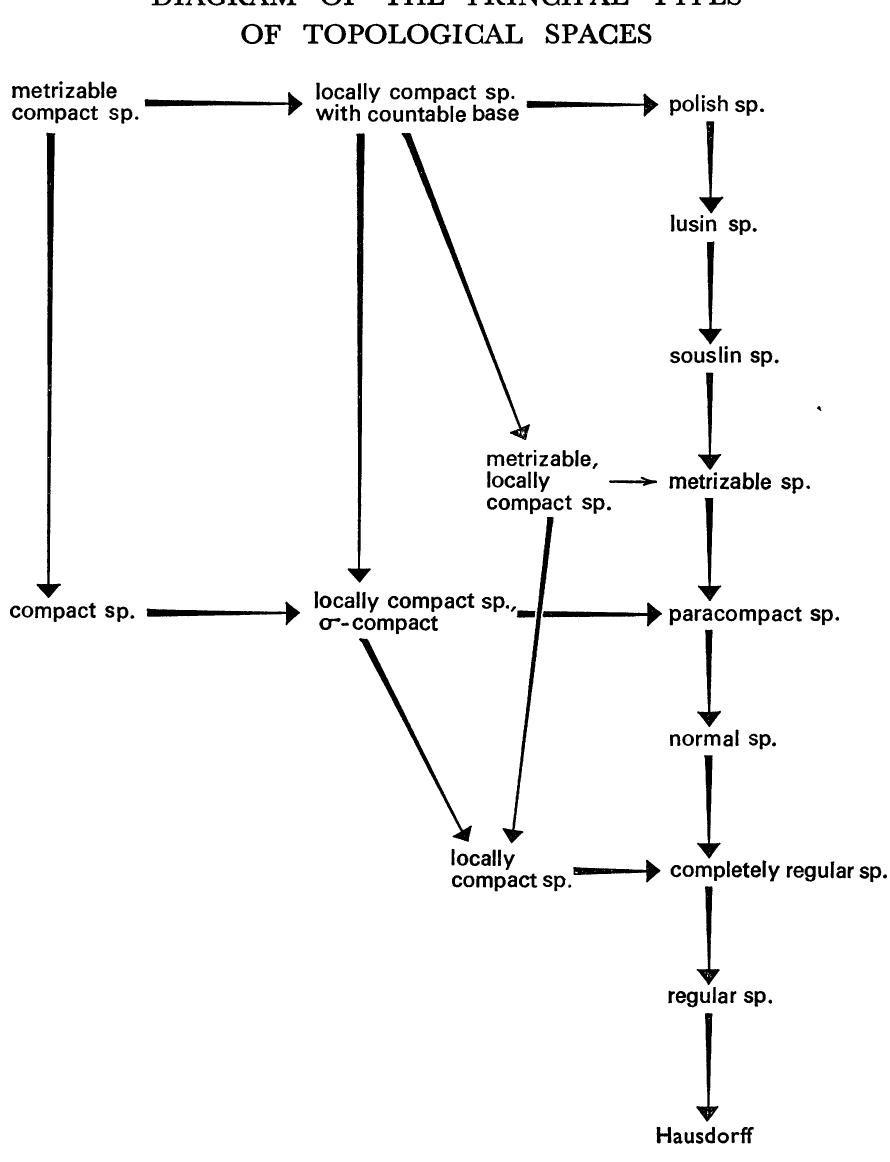
\includegraphics[keepaspectratio]{images/part002_2eb706e7.jpg}}

\section*{历史注记}
\phantomsection
\addcontentsline{toc}{section}{历史注记}

（括号中的数字指本注记末尾的参考文献。）

如我们在第 II 章的历史注记中所说，度量空间的概念是 M. Fréchet 于 1906 年引入的，几年后由 F. Hausdorff 在其``Mengenlehre''（《集论》）中加以发展。1920 年以后它获得了巨大的重要性，部分地是由于 S. Banach 及其学派关于赋范空间及其在泛函分析中的应用的基础性工作，也是由于绝对值概念在数论与代数几何中的重要性（在那里，关于一个绝对值的完备化过程特别地显示出是一种有力的工具）。

1920-1930 这十年间出现了一整系列关于度量空间性质的研究。这些由莫斯科学派进行的研究，特别着眼于寻求给定的拓扑可度量化的必要充分条件。这一思想运动凸显了正规空间概念的意义，该概念由 Tietze 于 1923 年定义，但其重要作用只是作为 Urysohn 关于连续实值函数扩张的工作{[}6{]}的结果才被认识到。除去单实变量函数这一平凡情形外，把定义在闭集上的连续实值函数扩张到整个空间的问题，最先（就平面的情形）由 H. Lebesgue{[}3{]}考虑；在 Urysohn 的决定性结果之前，它已由 H. Tietze{[}4{]}对度量空间解决。把这问题推广到取值于任意拓扑空间的函数，近年来在代数拓扑中获得了相当的重要性。最近的工作还表明，在这类问题中正规空间的概念不易处理，因为它容许太多``病态''的可能；它常常必须用更受限制的仿紧性概念来代替，后者是 J. Dieudonné 于 1944 年引入的{[}9{]}。在这一理论中，最值得注意的结果是 A. H. Stone 的定理{[}10{]}：每个可度量化空间都是仿紧的 (*)。

我们已经指出过（第 IV 章的历史注记），十九世纪末与二十世纪初（E. Borel、Baire、Lebesgue、Osgood、W. H. Young）关于 \(R^{n}\) 中点集的分类，以及关于通过迭代取极限过程（关于函数列）从连续函数得到的实值函数的分类与刻画的重要工作。人们很快认识到，度量空间——其 1910 年以后的发展主要是俄国与波兰学派的工作——构成了这类研究的自然领域。除其他方面外，度量空间的研究清楚地表明了贫集概念以及完备度量空间中稠密开集的可数交定理（ \(§\ 5,\ no.\ 3,\ Theorem\ 1\) ）在现代分析中所起的基本作用，该定理最先（相互独立地）由 Osgood{[}1{]}对实直线证明，并由 Baire{[}2{]}对空间 \(R^{n}\) 证明。

另一方面，Souslin 于 1917 年{[}5{]}在纠正 Lebesgue 的一个错误时证明了波莱尔集的连续像未必是波莱尔集；这引导他定义并研究更大的一类集，此后称为``解析集''或``苏斯林集''。Souslin 早逝之后，这项工作特别由 N. Lusin（其思想曾启发 Souslin 的工作）与波兰数学家们（见{[}7{]}与{[}8{]}）继续推进。这些集如今的重要性在于它们对积分理论（在那里，由于它们的特殊性质，可以进行对任意可测集而言不可能的构造）以及现代位势论的应用；在位势论中，关于苏斯林集可容性的基本定理（最近由 G. Choquet{[}11{]}证明）已显示出在种种应用中的丰富内容。

\subsection*{参考文献}

{[}1{]} W. Osgood, Non-uniform convergence and the integration of series term by term, Amer. Journ. of Math., 19 (1897), pp.~155-190.

{[}2{]} R. BAIRE, Sur les fonctions de variables réelles, Ann. di Mat. (3), 3 (1899), p.~i.

{[}3{]} H. LEBESGUE, Sur le problème des Dirichlet, Rend. Circ. mat. di Palermo, 24 (1907), pp.~371-402.

{[}4{]} H. TIETZE, Über Funktionen, die auf einer abgeschlossenen Menge stetig sind, J. de Crelle, 145 (1915), pp.~9-14.

{[}5{]} M. SOUSLIN, Sur une définition des ensembles mesurables B sans nombres transfinis, C. R. Acad. Sci., 164 (1917), pp.~88-91.

{[}6{]} P. URYSOHN, Über die Mächtigkeit der zusammenhängenden Mengen, Math. Ann., 94 (1925), p.~262.

{[}7{]} N. Lusin, Leçons sur les ensembles analytiques et leurs applications, Paris (Gauthier-Villars), 1930.

{[}8{]} K. KURATOWSKI, Topologie I, 2nd edition, Warszawa-Vrocaw, 1948.

{[}9{]} J. DIEUDONNÉ, Une généralisation des espaces compacts, Journ. de Math. (9), 23 (1944), pp.~65-76.

{[}10{]} A. H. STONE, Paracompactness and product spaces, Bull. Amer. Math. Soc., 54 (1948), pp.~977-982.

{[}11{]} G. CHOQUET, Theory of capacities, Ann. Inst. Fourier, 5 (1953-1954) pp.~131-295.

\ResumeMainChapters
\chapter{函数空间}

\section{\texorpdfstring{\(\mathfrak{S}\)-收敛的一致结构}{S-收敛的一致结构}}

记号。若 X 与 Y 是任意两个集，我们回忆 X 到 Y 的一切映射组成的集记作 \(\mathcal{F}(\mathbf{X};\mathbf{Y})\)，它可与乘积集 \(\mathbf{Y}^{\mathbf{x}}\) 等同（《集合论》，第 II 章，§ 5，第 2 号）。对 \(\mathcal{F}(\mathbf{X};\mathbf{Y})\) 的每个子集 H 与每个 \(x\in \mathbf{X}\)，我们将用 \(\mathrm{H}(x)\) 表示元素 \(u(x)\in \mathbf{Y}\)（当 \(u\) 取遍 H 时）组成的集。若 \(\Phi\) 是 \(\mathcal{F}(\mathbf{X};\mathbf{Y})\) 上的滤子基，我们用 \(\Phi (x)\) 表示由诸集 \(\mathrm{H}(x)\)（H 取遍 \(\Phi\)）组成的 Y 上的滤子基。最后，我们回忆，对每个 \(u\in \mathcal{F}(\mathbf{X};\mathbf{Y})\) 与 X 的每个子集 A，\(u|\mathrm{A}\) 表示 \(u\) 在 A 上的限制，它是 A 到 Y 中的映射；若 H 是 \(\mathcal{F}(\mathbf{X};\mathbf{Y})\) 的子集，则 H\textbar A 将表示限制 \(u|\mathrm{A}\)（函数 \(u\in \mathrm{H}\) 的）组成的集。

\subsection{一致收敛的一致结构}

设 X 是一个集，Y 是一致空间。对 Y 的每个围域 V，用 \(W(V)\) 表示 X 到 Y 中的映射的对 \((u, v)\) 中使 \((u(x), v(x)) \in V\)（对所有 \(x \in X\)）者组成的集。当 V 取遍 Y 的围域集时，诸集 \(W(V)\) 构成 F(X; Y) 上某个一致结构的围域基本系。因为它们显然满足公理 \((\mathrm{U}_{\mathrm{I}}^{\prime})\)（第 II 章，§ 1，第 1 号）；若 V 与 \(V'\) 是 Y 的两个使 \(V \subset V'\) 的围域，我们有 \(W(V) \subset W(V')\)，因而诸集 \(W(V)\) 满足 \((\mathrm{B}_{\mathrm{I}})\)（第 I 章，§ 6，第 3 号）；我们有 \(\widehat{W(V)} = W(\overline{V}^{-1})\)，故 \((\mathrm{U}_{\mathrm{II}}^{\prime})\) 满足；最后，关系式`` \((u(x), v(x)) \in V\)（对所有 \(x \in X\)）''与`` \((v(x), w(x)) \in V\)（对所有 \(x \in X\)）''蕴含关系式`` \((u(x), w(x)) \in V^{2}\)（对所有 \(x \in X\)）''；换言之，我们有 \(\widehat{W(V)} \subset W(\overline{V}^{2})\)，这就证明了 \((\mathrm{U}_{\mathrm{III}}^{\prime})\)。

定义 1 。在集 \(\mathcal{F}(\mathbf{X};\mathbf{Y})\) 上以子集 \(W(\mathbf{V})\)（其中 \(\mathbf{V}\) 取遍 \(\mathbf{Y}\) 的围域集）组成的集为围域基本系的一致结构，称为一致收敛的一致结构。它诱导的拓扑称为一致收敛的拓扑。若滤子 \(\Phi\)（\(\mathcal{F}(\mathbf{X};\mathbf{Y})\) 上的）关于这拓扑收敛于元素 \(u_0\)，则称 \(\Phi\) 一致收敛于 \(u_0\)。

注意 \(\mathcal{F}(\mathrm{X};\mathrm{Y})\) 上的一致收敛拓扑依赖于 Y 的一致结构，而不只是 Y 的拓扑（习题 4）。

把 \(\mathcal{F}(\mathbf{X};\mathbf{Y})\) 赋以一致收敛的一致结构所得的一致空间记作 \(\mathcal{F}_u(\mathbf{X};\mathbf{Y})\)。

\subsection{\texorpdfstring{\(\mathfrak{S}\)-收敛}{S-收敛}}

定义 2 。设 X 是一个集，Y 是一致空间，S 是 X 的子集组成的一个集。在 S 的集上一致收敛的一致结构，或简称 S-收敛的一致结构，是 F(X; Y) 上使限制映射 \(u \to u|A\)（F(X, Y) 到一致空间 \(\mathcal{F}_u(A; Y)\) 中的，其中 A 取遍 S）一致连续的最粗一致结构。把 F(X; Y) 赋以 S-收敛的一致结构所得的一致空间记作 \(\mathcal{F}_{\mathfrak{S}}(X; Y)\)。

\(\mathfrak{S}\)-收敛的一致结构所诱导的拓扑称为 \(\mathfrak{S}\)-收敛的拓扑；它是使所有映射 \(u \to u|A\)（\(\mathcal{F}(X; Y)\) 到 \(\mathcal{F}_u(A; Y) (A \in \mathfrak{S})\) 中的）都连续的最粗拓扑（第 II 章，§ 2，第 3 号，命题 4 的推论）。

滤子 \(\Phi\)（\(\mathcal{F}(\mathbf{X};\mathbf{Y})\) 上的）收敛于 \(u_{0}\)（关于 \(\mathfrak{S}\)-收敛的拓扑），当且仅当 \(u|\mathrm{A}\) 一致收敛于 \(u_{0}|\mathrm{A}\)（关于 \(\Phi\)，对所有 \(\mathrm{A}\in \mathfrak{S}\)）（第 I 章，§ 7，第 6 号，命题 10），因此称 \(\Phi\) 一致收敛于 \(u_{0}\)（在 \(\mathfrak{S}\) 的集上）。

滤子基 \(\Phi\)（\(\mathcal{F}_{\mathfrak{S}}(\mathbf{X};\mathbf{Y})\) 上的）是柯西滤子基，当且仅当对每个 \(\mathbf{A}\in\mathfrak{S}\)，\(\Phi\) 在映射 \(u\to u|\mathbf{A}\) 下的像是 \(\mathcal{F}_{u}(\mathbf{A};\mathbf{Y})\) 上的柯西滤子基（第 II 章，§ 3，第 1 号，命题 4）。

设 \(f\) 是拓扑（相应地，一致）空间 \(Z\) 到 \(\mathcal{F}_{\mathfrak{S}}(X; Y)\) 中的映射。则 \(f\) 连续（相应地，一致连续），当且仅当对每个 \(A \in \mathfrak{S}\)，映射 \(z \to f(z)|A\)（\(Z\) 到 \(\mathcal{F}_u(A; Y)\) 中的）连续（相应地，一致连续）（第 I 章，§ 2，第 3 号，命题 4；第 II 章，§ 2，第 3 号，命题 4）。

最后，设 \(\mathbf{M}\) 是 \(\mathcal{F}_{\mathfrak{S}}(\mathbf{X};\mathbf{Y})\) 的子集；则 \(\mathbf{M}\) 是准紧的，当且仅当对每个 \(\mathbf{A} \in \mathfrak{S}\)，限制 \(u|\mathbf{A}\)（\(u \in \mathbf{M}\)）组成的集是 \(\mathcal{F}_u(\mathbf{A};\mathbf{Y})\) 的准紧子集（第 II 章，§ 4，第 2 号，命题 3）。

注记。1) 初始一致结构的围域的一般定义（第 II 章，§ 2，第 3 号，命题 4）表明，\(\mathcal{F}_{\mathfrak{S}}(\mathrm{X};\mathrm{Y})\) 的围域基本系可如下得到：对每个 \(\mathbf{A}\in \mathfrak{S}\) 与每个围域 \(\mathbf{V}\)（\(\mathfrak{B}\) 的，此基本系属于 \(\mathbf{Y}\)），用 \(W(\mathbf{A},\mathbf{V})\) 表示映射的对 \((u,v)\)（\(\mathbf{X}\) 到 \(\mathbf{Y}\) 中的）中使 \((u(x),v(x))\in \mathbf{V}\)（对每个 \(x\in \mathbf{A}\)）者组成的集；当 \(\mathbf{A}\) 取遍 \(\mathfrak{S}\) 且 \(\mathbf{V}\) 取遍 \(\mathfrak{B}\) 时，诸集 \(W(\mathbf{A},\mathbf{V})\) 的有限交构成 \(\mathcal{F}_{\mathfrak{S}}(\mathrm{X};\mathrm{Y})\) 的围域基本系。

这描述立即表明：若 \(\mathfrak{S},\mathfrak{S}'\) 是 \(\mathbf{X}\) 的子集的两个集，使 \(\mathfrak{S} \subset \mathfrak{S}'\)，则 \(\mathfrak{S}'\)-收敛的一致结构比 \(\mathfrak{S}\)-收敛的一致结构更细。

\begin{enumerate}
\def\labelenumi{\arabic{enumi})}
\setcounter{enumi}{1}
\tightlist
\item
  然而，把 \(\mathfrak{S}\) 换成由含于 \(\mathfrak{S}\) 的集的有限并之中的 X 的所有子集组成的集 \(\mathfrak{S}'\)，\(\mathfrak{S}\)-收敛的一致结构不变。因此在研究 \(\mathfrak{S}\)-收敛时，我们总可以限于集 \(\mathfrak{S}\) 满足下列两个条件的情形：
\end{enumerate}

\((\mathbf{F}_{\mathbf{I}}^{\prime})\) \(\mathfrak{S}\) 中的集的每个子集都属于 \(\mathfrak{S}\)。

\((F_{\mathrm{II}}^{\prime})\) \(\mathfrak{S}\) 中的集的每个有限并都属于 \(\mathfrak{S}\)。

若 \((\mathbf{F}_{\mathrm{II}}^{\prime})\) 满足，则 \(\mathcal{F}_{\mathfrak{S}}(\mathbf{X};\mathbf{Y})\) 的一个围域基本系可这样得到：取所有集 \(\boldsymbol{W}(\mathrm{A},\mathrm{V})\)（其中 A 取遍 S，V 取遍 Y 的一个围域基本系）。

\begin{enumerate}
\def\labelenumi{\arabic{enumi})}
\setcounter{enumi}{2}
\tightlist
\item
  \(\mathfrak{S}\)-收敛的一致结构是这乘积空间的一致结构在映射 \(u \to (u|\mathbf{A})_{\mathbf{A} \in \mathfrak{S}}\)（\(\mathcal{F}(\mathbf{X}; \mathbf{Y})\) 到 \(\prod_{\mathbf{A} \in \mathfrak{S}} \mathcal{F}_u(\mathbf{A}; \mathbf{Y})\) 中的）下的逆像（第 II 章，§ 2，第 6 号，命题 8）。若 \(\mathfrak{S}\) 是 \(\mathbf{X}\) 的覆盖，则此映射是单射，因而 \(\mathcal{F}_{\mathfrak{S}}(\mathbf{X}; \mathbf{Y})\) 同构于 \(\prod_{\mathbf{A} \in \mathfrak{S}} \mathcal{F}_u(\mathbf{A}; \mathbf{Y})\) 的、作为此映射之像的一致子空间。
\end{enumerate}

命题 1 。若 Y 是豪斯多夫的且 S 是 X 的覆盖，则空间 \(\mathcal{F}_{\mathfrak{S}}(X;Y)\) 是豪斯多夫的。

设 \(u, v\) 是 \(\mathcal{F}_{\mathfrak{S}}(\mathrm{X}; \mathrm{Y})\) 的两个元素，使 \((u, v) \in W(\mathrm{A}, \mathrm{V})\)（对每个围域 \(\mathrm{V}\)（\(\mathrm{Y}\) 的）与每个 \(\mathrm{A} \in \mathfrak{S}\)）。由于 \(\mathrm{Y}\) 是豪斯多夫的，推出 \(u\) 与 \(v\) 在每个集 \(\mathrm{A} \in \mathfrak{S}\) 上一致；又因 \(\mathfrak{S}\) 覆盖 \(\mathrm{X}\)，必有 \(u = v\)。

注记。4) 设 H 是 \(\mathcal{F}(\mathbf{X};\mathbf{Y})\) 的子集。滥用术语，把 \(\mathfrak{S}\)-收敛的一致结构（相应地，拓扑）（\(\mathcal{F}(\mathbf{X};\mathbf{Y})\) 上的）在 H 上诱导的一致结构（相应地，拓扑）称为集 H 上 \(\mathfrak{S}\)-收敛的一致结构（相应地，拓扑）。

\begin{enumerate}
\def\labelenumi{\arabic{enumi})}
\setcounter{enumi}{4}
\tightlist
\item
  设 L 是由滤子 \(\mathfrak{G}\) 滤化的集，且 \(\lambda \to u_{\lambda}\) 是 L 到 \(\mathcal{F}_{\mathfrak{S}}(\mathbf{X};\mathbf{Y})\) 中的、有极限 \(v\)（关于 \(\mathfrak{G}\)）的映射；这时我们说，关于滤子 \(\mathfrak{G}\)，X 到 Y 中的映射 \(u_{\lambda}\) 一致收敛于 \(v\){[}或族 \((u_{\lambda})\) 一致收敛于 \(v\){]}（在 \(\mathfrak{S}\) 的每个集上）。若 \(\mathbf{L} = \mathbf{N}\) 且 \(\mathfrak{G}\) 是弗雷歇滤子，则在这陈述中省略对 \(\mathfrak{G}\) 的提及。
\end{enumerate}

更特殊地，设 Y 上定义了一个交换且结合的、以加法记号书写的合成律。若 \((u_{n})\) 是 X 到 Y 中的映射的任一序列，用 \(v_{n}\) 表示由下式定义的映射

\[
v _ {n} (x) = \sum_ {k = 0} ^ {n} u _ {k} (x) \quad (n \in \mathbf {N});
\]

我们说以 \(u_n\) 为通项的级数在 \(\mathfrak{S}\) 的每个集上一致收敛，如果序列 \((v_n)\) 在 \(\mathfrak{S}\) 的每个集上一致收敛。类似地，映射的一致可和族 \((u_\lambda)_{\lambda \in \mathbf{L}}\)（\(\mathbf{X}\) 到 \(\mathbf{Y}\) 中的）通过考虑映射 \(x \to \sum_{\lambda \in \mathbf{J}} u_\lambda(x)\)（对 L 的所有有限子集

J）以及这些映射在 \(\mathcal{F}_{\mathfrak{S}}(\mathbf{X};\mathbf{Y})\) 中关于 L 的有限子集的定向集的极限来定义（第 III 章，§ 5，第 1 号）。

\begin{enumerate}
\def\labelenumi{\arabic{enumi})}
\setcounter{enumi}{5}
\tightlist
\item
  由定义 1 与定义 2 立即得出：对每个 \(x \in \bigcup_{\mathbf{A} \in \mathfrak{S}} \mathbf{A}\)，映射 \(u \to v(x)\)（\(\mathcal{F}_{\mathfrak{S}}(\mathbf{X}; \mathbf{Y})\) 到 Y 中的）是一致连续的。因而特别地，若用 \(\overline{\mathbf{H}}\) 表示 \(\mathcal{F}_{\mathfrak{S}}(\mathbf{X}; \mathbf{Y})\) 的子集 H 的闭包，则有 \(\overline{\mathbf{H}}(x) \subset \overline{\mathbf{H}(x)}\)（对所有 \(x \in \bigcup_{\mathbf{A} \in \mathfrak{S}} \mathbf{A}\)）（第 I 章，§ 2，第 1 号，定理 1）。
\end{enumerate}

\subsection{\texorpdfstring{\(\mathfrak{S}\)-收敛的例子}{S-收敛的例子}}

I. 在 X 的子集上的一致收敛。设 A 是 X 的子集，取 \(\mathfrak{S} = \{\mathrm{A}\}\)。\(\mathfrak{S}\)-收敛的一致结构（相应地，拓扑）这时称为在 A 中一致收敛的一致结构（相应地，拓扑）；若滤子 \(\Phi\)（\(\mathcal{F}_{\mathfrak{S}}(\mathrm{X};\mathrm{Y})\) 上的）收敛于 \(u_0\)，则称它在 A 中一致收敛于 \(u_0\)。当 \(\mathrm{A} = \mathrm{X}\) 时，我们重新得到第 1 号中定义的一致收敛结构。

\begin{enumerate}
\def\labelenumi{\Roman{enumi}.}
\setcounter{enumi}{1}
\tightlist
\item
  在 X 的子集上的逐点收敛。设 A 是 X 的子集，取 S 为由属于 A 的单个点组成的 X 的所有子集之集（由第 2 号的注记 2，若取 S 为 A 的所有有限子集之集，效果相同）。S-收敛的一致结构（相应地，拓扑）这时称为在 A 中逐点收敛的一致结构（相应地，拓扑）；若 \(\mathcal{F}_{\mathfrak{S}}(\mathbf{X};\mathbf{Y})\) 上的滤子 Φ 收敛于 \(u_0\)，则称它在 A 中逐点收敛于 \(u_0\)。这种情形成立当且仅当：对每个 \(x\in \mathbf{A}\)，\(u_0(x)\) 是 \(u(x)\) 关于滤子 Φ 的极限。
\end{enumerate}

特别地，当 A = X 时，在 X 中逐点收敛的一致结构（相应地，拓扑）就简称为逐点收敛的一致结构（相应地，拓扑）；把 \(\mathcal{F}(X; Y)\) 赋以这结构所得的一致空间记作 \(\mathcal{F}_{s}(X; Y)\)。注意逐点收敛的拓扑就是 \(Y^{X}\) 上的乘积拓扑，因而只依赖于 Y 的拓扑而不依赖其一致结构。

\begin{enumerate}
\def\labelenumi{\Roman{enumi}.}
\setcounter{enumi}{2}
\tightlist
\item
  紧收敛。设 X 是拓扑空间，取 S 为 X 的所有紧子集组成的集。这时 S-收敛的一致结构（相应地，拓扑）称为紧收敛的一致结构（相应地，拓扑），而赋予 \(\mathcal{F}(X;Y)\) 此一致结构所得的一致空间记作 \(\mathcal{F}_{c}(X;Y)\)。紧收敛的结构比一致收敛的结构粗，且当 X 紧时二者一致；它又比逐点收敛的结构细，且当 X 离散时这二者一致。
\end{enumerate}

若 X 是一致空间，则通过取 S 为 X 的所有准紧子集组成的集，我们可以在 \(\mathcal{F}(X;Y)\) 上定义准紧收敛的一致结构。同样，若 X 是度量空间，则可取 S 为 X 的所有有界子集组成的集；这时 S-收敛的一致结构称为有界收敛的一致结构。

\subsection{\texorpdfstring{空间 \(\mathcal{F}_{\mathfrak{G}}(\mathbf{X};\mathbf{Y})\) 的性质}{空间 F 下标 G (X;Y) 的性质}}

命题 2. 设 \(\mathbf{X}_1, \mathbf{X}_2\) 是两个集，\(\mathbf{Y}\) 是一致空间，\(\mathfrak{S}_i\) 是 \(\mathbf{X}_i\) 的子集组成的集（\(i = 1, 2\)），而 \(\mathfrak{S}_1 \times \mathfrak{S}_2\) 是 \(\mathbf{X}_1 \times \mathbf{X}_2\) 的形如 \(\mathbf{A}_1 \times \mathbf{A}_2\) 的子集组成的集，其中 \(\mathbf{A}_i \in \mathfrak{S}_i\)（\(i = 1, 2\)）。则典范双映射

\[
\mathscr {F} \left(\mathrm{X} _ {1} \times \mathrm{X} _ {2}; \mathrm{Y}\right)\rightarrow \mathscr {F} \left(\mathrm{X} _ {1}; \mathscr {F} \left(\mathrm{X} _ {2}; \mathrm{Y}\right)\right)
\]

（集合论，R，§ 4，第 14 号）是一致空间

\[
\mathcal {F} _ {\mathfrak {S} _ {1} \times \mathfrak {S} _ {2}} (\mathrm{X} _ {1} \times \mathrm{X} _ {2}; \mathrm{Y})
\]

到 \(\mathcal{F}_{\mathfrak{S}_1}(\mathbf{X}_1;\mathcal{F}_{\mathfrak{S}_2}(\mathbf{X}_2;\mathbf{Y}))\) 上的同构

设 \(\mathbf{V}\) 是 \(\mathbf{Y}\) 的围域，\(\mathbf{A}_i\in \mathfrak{S}_i\)（\(i = 1,2\)）；则由定义立即可见，\(W(\mathbf{A}_1\times \mathbf{A}_2,\mathbf{V})\) 经典范双映射与 \(W(\mathbf{A}_1,W(\mathbf{A}_2,\mathbf{V}))\) 等同，结论立得。

命题 3. a) 设 X 是一个集；S 是 X 的子集组成的一个集；Y、Y' 是两个一致空间；f: Y → Y' 是一致连续映射。则 F\_S(X; Y) 到 F\_S(X; Y') 中的映射 u → f ∘ u 是一致连续的。

\begin{enumerate}
\def\labelenumi{\alph{enumi})}
\setcounter{enumi}{1}
\tightlist
\item
  设 \(\mathbf{X}, \mathbf{X}'\) 是两个集；\(\mathfrak{S}\)（相应地，\(\mathfrak{S}'\)）是 \(\mathbf{X}\)（相应地，\(\mathbf{X}'\)）的子集组成的集；\(\mathbf{Y}\) 是一致空间；\(g: \mathbf{X}' \to \mathbf{X}\) 是这样的映射：对每个 \(\mathbf{A}' \in \mathfrak{S}'\)，\(g(\mathbf{A}')\) 含于 \(\mathfrak{S}\) 中集的有限并。则映射 \(u \to u \circ g\)（\(\mathcal{F}_{\mathfrak{S}}(\mathbf{X}, \mathbf{Y})\) 到 \(\mathcal{F}_{\mathfrak{S}'}(\mathbf{X}', \mathbf{Y})\) 中的）是一致连续的。
\end{enumerate}

命题 4. 设 X、Y 是两个集，\((\mathbf{X}_{\lambda})_{\lambda \in \mathbf{L}}\) 是一个集族，\((\mathrm{Y}_{\mu})_{\mu \in \mathbf{M}}\) 是一个一致空间族。对每个 \(\lambda \in \mathbf{L}\)，设 \(\mathfrak{S}_{\lambda}\) 是 \(\mathbf{X}_{\lambda}\) 的子集组成的集，\(g_{\lambda}\) 是 \(\mathbf{X}_{\lambda}\) 到 X 中的映射，而 \(\mathfrak{S}\) 是 X 的子集组成的集，即诸集 \(g_{\lambda}(\mathfrak{S}_{\lambda})\) 的并。对每个 \(\mu \in \mathbf{M}\)，设 \(f_{\mu}\) 是 Y 到 \(Y_{\mu}\) 中的映射，并赋予 Y 使诸 \(f_{\mu}\) 都一致连续的最粗一致结构。则 \(\mathcal{F}(X;Y)\) 上 S-收敛的一致结构是使映射 \(u \to f_{\mu} \circ u \circ g_{\lambda}\)（\(\mathcal{F}(X;Y)\) 到 \(\mathcal{F}_{\mathfrak{S}_{\lambda}}(X_{\lambda},Y_{\mu})\) 中的）都一致连续的最粗一致结构。

这些命题是第 2 号注记 1 中给出的 S-收敛的一致结构的围域基本系描述的直接推论；证明的细节留给读者。特别地，命题 4 蕴含：

推论. 设 X 是一个集，\((\mathrm{Y}_{t})_{t\in\mathbf{I}}\) 是一致空间族，S 是 X 的子集组成的集。若赋予 \(\prod_{t\in I}Y_{t}\) 乘积一致结构，则一致空间 \(\mathcal{F}_{\mathfrak{S}}\left(\mathrm{X},\prod_{t\in\mathbf{I}}\mathrm{Y}_{t}\right)\) 到乘积一致空间 \(\prod_{t\in\mathbf{I}}\mathcal{F}_{\mathfrak{S}}(\mathrm{X};\mathrm{Y}_{t})\) 上的典范双映射（集合论，R，§ 4，第 13 号）是同构。

\subsection{\texorpdfstring{\(\mathcal{F}_{\mathfrak{S}}(\mathbf{X};\mathbf{Y})\) 的完全子集}{F 下标 S (X;Y) 的完全子集}}

命题 5. 设 \(\Phi\) 是一个集，Y 是一致空间，\(\mathfrak{S}\) 是 X 的子集组成的集。则滤子 \(\Phi\)（\(\mathcal{F}_{\mathfrak{S}}(\mathbf{X};\mathbf{Y})\) 上的）收敛于 \(u_0\) 的充要条件是：\(\Phi\) 是关于 \(\mathfrak{S}\) -收敛的一致结构的柯西滤子，且逐点收敛于 \(u_0\)（在 \(\mathbf{B} = \bigcup_{\mathbf{A}\in \mathfrak{S}}\mathbf{A}\) 中）。

由于 B 中逐点收敛的结构比 S-收敛的结构粗，只需证明：对每个 \(A \in S\) 与 Y 的每个闭围域 V，\(W(A, V)\) 关于逐点收敛拓扑在 B 中是闭的（第 II 章，§ 3，第 3 号，命题 7）。而 \(W(A, V)\) 是诸映射 \((u, v) \to (u(x), v(x))\)（当 x 取遍 A 时）下 V 的原象的交；这些映射关于逐点收敛拓扑连续（第 2 号注记 6），由此即得结论。

推论 1. \(\mathcal{F}_{\mathfrak{S}}(\mathbf{X};\mathbf{Y})\) 的子空间 H 是完全的，充要条件是：对 H 上每个柯西滤子 \(\Phi\)，存在 \(u_0\in \mathbf{H}\)，使 \(\Phi\) 逐点收敛于 \(u_0\)（在 \(\mathbf{B} = \bigcup_{\mathbf{A}\in \mathfrak{S}}\mathbf{A}\) 中）。

这由命题 5 立得。

推论 2. 设 \(\mathfrak{S}_1, \mathfrak{S}_2\) 是 X 的子集组成的两个集，它们的并相同，且 \(\mathfrak{S}_1 \subset \mathfrak{S}_2\)，又设 H 是 \(\mathcal{F}(X; Y)\) 的子集。则若 H 关于 \(\mathfrak{S}_1\) -收敛是完全的，它关于 \(\mathfrak{S}_2\) -收敛也是完全的。

因为关于 \(S_{2}\) -收敛的每个柯西滤子也是关于 \(S_{1}\) -收敛的柯西滤子，故可应用推论 1。

推论 3. 设 H 是 \(\mathcal{F}(\mathbf{X};\mathbf{Y})\) 的子集，使得对每个

\[
x \notin \mathrm{B} = \bigcup_ {\mathrm{A} \in \mathfrak {S}} \mathrm{A},
\]

\(\mathbf{H}(x)\) 在 \(\mathbf{Y}\) 中的闭包是 \(\mathbf{Y}\) 的完全子空间。则 \(\overline{\mathbf{H}}\)（即 \(\mathbf{H}\) 在 \(\mathcal{F}_{\mathfrak{S}}(\mathbf{X};\mathbf{Y})\) 中的闭包）是完全子空间。

设 \(\Phi\) 是 \(\overline{\mathbf{H}}\) 上的柯西滤子，如下定义映射 \(v: \mathbf{X} \to \mathbf{Y}\)。若 \(x \in \mathbf{B}\)，则 \(\Phi(x)\) 是 \(\overline{\mathbf{H}(x)}\) 上的柯西滤子（第 2 号注记 6），故由假设它至少有一个极限点；取 \(v(x)\) 为这些极限之一。若 \(x \notin \mathbf{B}\)，取 \(v(x)\) 为 \(\mathbf{Y}\) 的任意一点。以如此定义的 \(v\)，显然 \(\Phi\) 逐点收敛于 \(v\)（在 \(\mathbf{B}\) 中），因而由命题 5，\(v\) 是 \(\Phi\) 在 \(\mathcal{F}_{\mathfrak{S}}(\mathbf{X}; \mathbf{Y})\) 中的一个极限。

特别地，若 Y 是完全的，则命题 5 的推论 3 的假设对每个 \(H \subset \mathcal{F}(X; Y)\) 都满足；因此：

定理 1. 设 X 是一个集，S 是 X 的子集组成的一个集，Y 是完全一致空间。则一致空间 \(\mathcal{F}_{\mathfrak{S}}(X;Y)\) 是完全的。
